\chapter{'തറവാട്ടിൽ പിറന്നവളും' 'ചന്തപ്പെണ്ണും' ഉണ്ടായതെങ്ങനെ?}
\label{chapter4}
\begin{figure}[h]
\begin{center}
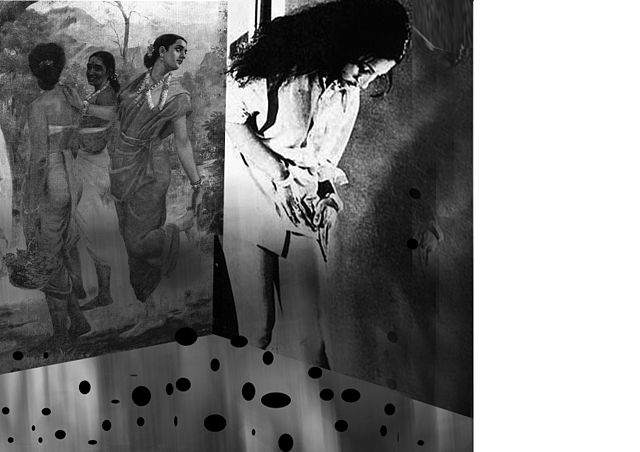
\includegraphics[width=\textwidth,height=8cm]{Kulasthree_Chapter_four_pic01.jpg}
\end{center}
%\caption*{പുലയർ - കെ പി പത്മനാഭ മേനോൻ - വാള്യം 3, (1929), 1984}
\end{figure}

\paragraph{}പത്തൊമ്പതാം നൂറ്റാണ്ടിന്റെ അവസാനദശകങ്ങൾ മുതൽ സമുദായപരിഷ്കരണപ്രസ്ഥാനങ്ങൾ ശക്തിപ്രാപിച്ചതോടുകൂടി പരമ്പരാഗത ജാതിസമൂഹങ്ങളുടെ തിരോധാനം ആരംഭിച്ചുവെന്ന് നമുക്കറിയാം. പരമ്പരാഗത ലിംഗമൂല്യങ്ങൾ മനുഷ്യത്വത്തിനെതിരാണെന്ന വിമർശനമുന്നയിച്ച ഈ പ്രസ്ഥാനങ്ങൾ അവയ്ക്കു പകരം പുതിയ മൂല്യങ്ങളെ മുന്നോട്ടുവച്ചു. ഇന്നു നമുക്കു പരിചിതങ്ങളായ ആൺ-പെൺഭേദങ്ങളും ഇരട്ടസദാചാരവും രൂപംപ്രാപിച്ചത് ഈ കാലഘട്ടത്തിലാണ്. സ്ത്രീകൾക്കിടയിൽത്തന്നെ 'നല്ല' സ്ത്രീയെയും 'ചീത്ത' സ്ത്രീയെയും വേർതിരിക്കുന്ന മാനദണ്ഡങ്ങൾ ഇതിന്റെ ഭാഗമായിരുന്നു. സ്ത്രീകളെ കുടുംബത്തിനുള്ളിലും സമൂഹത്തിലും സക്രിയരാക്കിത്തീർക്കാനുള്ള പരിശ്രമങ്ങളിലൂടെത്തന്നെയാണ് സ്ത്രീകളെ രണ്ടാംതരക്കാരാക്കി ചുരുക്കിയ ഈ മൂല്യങ്ങൾ വളർന്നുവികസിച്ചത്.

\section{നവവരേണ്യതയുടെ ലിംഗമൂല്യങ്ങൾ}
\label{ch4sec1}
\paragraph{}
കേരളത്തിൽ സ്ത്രീകളെ വിശേഷിപ്പിക്കാൻ ഉപയോഗിക്കുന്ന രണ്ടു പ്രയോഗങ്ങളാണിവ - 'തറവാട്ടിൽ പിറന്നവൾ', 'ചന്തപ്പെണ്ണ്'. 'മാന്യതയുള്ള സ്ത്രീ'യെ 'തറവാട്ടിൽ പിറന്നവൾ' എന്നു വിശേഷിപ്പിക്കുമ്പോൾ 'മാന്യതയില്ലാത്ത സ്ത്രീ'യെ 'ചന്തപ്പെണ്ണ്' എന്നു വിളിക്കുന്നു. ഈ വിളിയിൽ പഴയ ജാതിവ്യവസ്ഥയുടെ അംശങ്ങൾ പതിയിരിക്കുന്നുണ്ടെന്നു തീർച്ച. 'തറവാട്' എന്നാൽ പഴയ ജാത്യാഭിമാനത്തിന്റെ കേന്ദ്രമായിരുന്നല്ലോ. 'ചന്ത'യോ? പല ജാതിക്കാർ, പ്രത്യേകിച്ചു കീഴ്ജാതിക്കാർ, പല മതക്കാർ, ആണും പെണ്ണും ഒത്തുചേരുന്ന, 'ജാതിശുദ്ധം' തീരെ പാലിക്കാൻ പറ്റാത്ത ഇടമാണ്! അപ്പോൾ തറവാട്ടിലിരിക്കുന്നവൾ പരിശുദ്ധയും ചന്തയിൽ പണിയെടുക്കുന്നവൾ അശുദ്ധയുമായി കണക്കാക്കപ്പെട്ടത് സ്വാഭാവികം മാത്രം! പക്ഷേ, പരമ്പരാഗതമൂല്യവ്യവസ്ഥയ്ക്ക് 20-ാം നൂറ്റാണ്ടിൽ വൃദ്ധിയല്ല, ക്ഷയമാണ് സംഭവിച്ചതെന്ന് നമുക്കറിയാം. സമൂഹത്തിന്റെ മേൽത്തട്ടിലേക്ക് ഉയർന്നുവരാൻ വ്യക്തികളുടെ മുന്നിൽ നിരവധി വഴികൾ തുറന്നുകിട്ടിയ കാലമായിരുന്നു ഇത് - തറവാടിന്റെ മേൽവിലാസത്തിനുപുറമെ ഉന്നതവിദ്യാഭ്യാസം, ഉയർന്ന സാമ്പത്തികസ്ഥിതി, ഉദ്യോഗപദവി മുതലായവ സാമൂഹ്യമായ കയറ്റം നേടാനുള്ള മാർഗ്ഗങ്ങളായി ഇക്കാലത്തുയർന്നുവന്നു. നമ്മുടെ ഭാഷയിൽ, പക്ഷേ, ഇന്നും ഇത്തരം പ്രയോഗങ്ങൾ നിലനിൽക്കുന്നു. ജാതിപാരമ്പര്യത്തിന്റെ അവശിഷ്ടം മാത്രമാണോ ഇത്? പഴയ ജാതിസമുദായത്തിലെ പ്രമാണികൾക്കു പകരം 19-ാം നൂറ്റാണ്ടിലെ പുതിയ സാദ്ധ്യതകൾ പ്രയോജനപ്പെടുത്തിയ കൂട്ടരിൽനിന്നുണ്ടായ വർഗ്ഗം - 'നവവരേണ്യർ' എന്ന് നമുക്കവരെ വിളിക്കാം - പഴയ മൂല്യങ്ങളിൽ പലതിനേയും തള്ളിക്കളഞ്ഞു; പല പുതിയ മൂല്യങ്ങളെയും പരിപോഷിപ്പിച്ചു. എന്നാൽ, പഴയ വരേണ്യതയെ ഒന്നടങ്കം ഉപേക്ഷിച്ചുകൊണ്ടല്ല നവവരേണ്യർ തങ്ങളുടെ പുതിയ മൂല്യവ്യവസ്ഥയ്ക്കു രൂപംകൊടുത്തത്. പുതിയ മൂല്യങ്ങൾ സ്വീകരിക്കുന്നതിനുപുറമെ പഴയ വരേണ്യമൂല്യങ്ങളിൽനിന്ന് ചിലതുമാത്രം തെരഞ്ഞെടുത്ത് പരിഷ്ക്കരിച്ചുകൊണ്ടുകൂടിയാണ് നവവരേണ്യർ തങ്ങളുടെ മൂല്യവ്യവസ്ഥ ഉണ്ടാക്കിയത്.

\paragraph{}
\begin{wrapfigure}{i}{0.4\textwidth}
%\begin{figure}
%\begin{center}
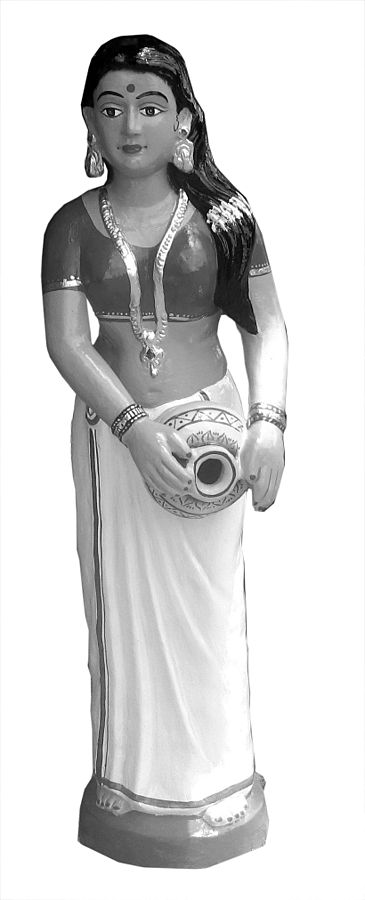
\includegraphics[width=0.4\textwidth,height=10cm]{Kulasthree_Chapter_four_pic02.jpg}
%\end{center}
%\caption*{പുലയർ - കെ പി പത്മനാഭ മേനോൻ - വാള്യം 3, (1929), 1984}
\end{wrapfigure}ആരായിരുന്നു, ഈ 'നവവരേണ്യർ'? 19-ാം നൂറ്റാണ്ടിലെ കേരളത്തിൽ, വിശേഷിച്ചും തിരുവിതാംകൂർ-കൊച്ചി പ്രദേശങ്ങളിൽ, നിരവധി കാതലായ സാമൂഹ്യസാമ്പത്തികമാറ്റങ്ങളുണ്ടായി. ബ്രിട്ടിഷ് അധികാരം നിലവിൽവന്നതോടെ ഈ രാജ്യങ്ങളിലെ ഭരണസംവിധാനങ്ങളെ നവീകരിക്കാനുള്ള ശ്രമമാരംഭിച്ചു. മിഷണറിമാരും പിൽക്കാലത്ത് സർക്കാരുകളും പ്രചരിപ്പിച്ച നവീനവിദ്യാഭ്യാസത്തിലൂടെ സർക്കാർ ഉദ്യോഗങ്ങളും പദവികളും നേടാമെന്നുവന്നു. പുതിയ വിദ്യാലയങ്ങളും കലാലയങ്ങളും സ്ഥാപിക്കപ്പെട്ടുതുടങ്ങി - അവിടങ്ങളിലും ഇംഗ്ലിഷ്‌വിദ്യാഭ്യാസം നേടിയവർക്കു ജോലിസാദ്ധ്യത തെളിഞ്ഞു. വ്യാപരരംഗം സജീവമായതോടുകൂടി അഭ്യസ്തവിദ്യർക്ക് അവിടെയും തൊഴിലവസരങ്ങൾ വർദ്ധിച്ചു. വ്യാപാരപ്രമുഖർ, വ്യവസായികൾ, അദ്ധ്യാപകർ, സർക്കാർ ഉദ്യോഗസ്ഥർ തുടങ്ങിയ കൂട്ടരടങ്ങിയ ഈ പുതിയ ജനവിഭാഗം 19-ാം നൂറ്റാണ്ടിന്റെ അവസാനദശകങ്ങളിൽ തിരുവിതാംകൂറിലും കൊച്ചിയിലും മലബാറിലും സജീവസാന്നിദ്ധ്യമായി. ആധുനിക പൊതുമണ്ഡലം ഇവരിലൂടെയാണ് രൂപപ്പെട്ടത് - അതായത് പത്രമാസികകൾ, ചർച്ചാവേദികൾ, വായനാസംഘങ്ങൾ മുതലായവ കൂടിച്ചേരുന്ന, സമൂഹത്തിന്റെ പൊതുപ്രശ്നങ്ങൾ ചർച്ചചെയ്യപ്പെടുന്ന, പുതിയ ഒരിടം ഇവരുടെ പ്രവർത്തനങ്ങളിലൂടെ രൂപപ്പെട്ടുതുടങ്ങി. അതുപോലെ, സ്വന്തം സമുദായങ്ങളെ കാലത്തിനൊത്ത് പരിഷ്ക്കരിക്കേണ്ടതെങ്ങനെ എന്ന ചോദ്യം ആദ്യമുന്നയിച്ചത് ആ സമുദായങ്ങളിലെ നവവരേണ്യർതന്നെ. മലബാറിലെ നായന്മാരിൽനിന്ന് സി. ശങ്കരൻനായർ, മാപ്പിളസമുദായത്തിൽനിന്ന് സനാ ഉല്ലാഹ് മക്തി തങ്ങൾ, തീയ്യ സമുദായത്തിൽനിന്ന് മൂർക്കോത്തു കുമാരൻ, കൊച്ചിയിലെ അരയസമുദായത്തിൽനിന്ന് പണ്ഡിറ്റ് കറുപ്പൻ, തിരുവിതാംകൂറിലെ ഈഴവരിൽനിന്ന് ഡോ.പൽപു, സുറിയാനി ക്രിസ്ത്യാനികൾക്കിടയിൽനിന്ന് പി.കെ. കൊച്ചീപ്പൻ തരകൻ തുടങ്ങിയ ആദ്യകാല സമുദായപരിഷ്ക്കർത്താക്കളും വക്താക്കളുമായിരുന്നവരെല്ലാം നവവരേണ്യരായിരുന്നു. ഇവരിൽ നല്ലൊരുവിഭാഗം പരമ്പരാഗത ജാതിവ്യവസ്ഥയിൽ മുന്തിയ സ്ഥാനമുണ്ടായിരുന്ന ജാതികളിൽ - അതായത്, നായർ - സുറിയാനി ക്രിസ്ത്യാനി ജാതികളിൽ - ഉൾപ്പെട്ടവരായിരുന്നു. ഇവരെക്കൂടാതെ തൊട്ടുകൂടാത്തവരായി ഗണിച്ചിരുന്ന ഈഴവ-തീയ്യ വിഭാഗങ്ങളിൽനിന്നും നവവരേണ്യരുണ്ടായിത്തുടങ്ങി. അതേസമയം പരമ്പരാഗതജാതിക്രമത്തിൽ മദ്ധ്യജാതികളിൽപ്പെട്ടിരുന്ന അരയസമുദായത്തിൽനിന്നും അധികംപേർ നവവരേണ്യവിഭാഗത്തിലേക്കു കടന്നില്ല. ഇരുപതാം നൂറ്റാണ്ടിൽ കേരളത്തിലുണ്ടായ സാമൂഹ്യ - രാഷ്ട്രീയ മാറ്റങ്ങളിൽനിന്നുള്ള നേട്ടങ്ങളധികവും കൊയ്തത് ഈ നവവരേണ്യവിഭാഗമായിരുന്നു.


\paragraph{}പൊതുവെ, മുതലാളിത്തവ്യവസ്ഥയുടെ സ്വത്തുനിയമങ്ങളോടുള്ള (അതായത് സ്വകാര്യസ്വത്തുടമസ്ഥതയ്ക്ക് അനുകൂലമായ നിയമങ്ങളോടുള്ള) കൂറ്, വ്യക്തികളുടെ സാമ്പത്തികവളർച്ചയിലൂടെയാണ് സമൂഹം പുരോഗമിക്കുന്നതെന്ന വിശ്വാസം, വ്യക്തികൾക്ക് മത്സരബുദ്ധിയോടെയുള്ള സാമ്പത്തികപ്രവർത്തനം നടത്താനുള്ള സാഹചര്യം ഒരുക്കലാണ് സമുദായപരിഷ്ക്കരണത്തിന്റെ ലക്ഷ്യമെന്ന വിശ്വാസം - ഇവ ഏറിയോ കുറഞ്ഞോ നവവരേണ്യമൂല്യവ്യവസ്ഥയിൽ ഉൾപ്പെട്ടിരുന്നു. ഈ മൂല്യങ്ങളെല്ലാംതന്നെ പാശ്ചാത്യലോകത്തുനിന്ന് ഇങ്ങോട്ടു പ്രവഹിച്ചവയായിരുന്നു. എന്നാൽ ഇവയോടൊപ്പം മറ്റുപല ആശയങ്ങളും പാശ്ചാത്യരാജ്യങ്ങളിൽനിന്ന് ഇവിടേക്കെത്തിയിരുന്നു. മനുഷ്യർ തമ്മിലുള്ള അടിസ്ഥാനപരമായ തുല്യത, സമത്വം, സാഹോദര്യം - ഈ ആശയങ്ങളും പാശ്ചാത്യലോകത്തുനിന്ന് ഇവിടെ എത്തിയവയാണ്. ഇവയ്ക്ക്, പക്ഷേ, ഭാഗികമായ അംഗീകാരമേ നവവരേണ്യർ നൽകിയുള്ളൂ. അഥവാ, നവവരേണ്യരുടെ താൽപര്യങ്ങൾക്ക് കോട്ടംതട്ടാത്തവിധത്തിൽമാത്രമേ അവ പ്രയോഗിക്കപ്പെട്ടുള്ളൂ. ശ്രീനാരായണഗുരുവിനെപ്പോലുള്ളവരുടെ സമത്വചിന്തയെപ്പോലും ഇത്തരത്തിൽ ന്യൂനീകരിക്കാൻ നവവരേണ്യർക്കു കഴിഞ്ഞു.

\paragraph{}
അതുകൊണ്ടുതന്നെ പാശ്ചാത്യലോകത്ത് വിമോചനകരങ്ങളായി വ്യാഖ്യാനിക്കപ്പെട്ട പല ആശയങ്ങളും ഇവിടെ തീരെ ചർച്ചചെയ്യപ്പെട്ടില്ല; അല്ലെങ്കിൽ ന്യൂനീകരിക്കപ്പെട്ടു. എന്തായാലും നവവരേണ്യർക്ക് അനുകൂലമായ വിധത്തിൽ പാശ്ചാത്യ ആശയങ്ങളെയും പ്രയോഗങ്ങളെയും എങ്ങനെ മാറ്റിത്തീർക്കാമെന്ന വിചാരം 20-ാം നൂറ്റാണ്ടിലെ ചർച്ചകളിൽ വ്യക്തമായും കാണാനുണ്ട്. ഉദാഹരണത്തിന്, 1930കൾമുതൽ ഇവിടെയാരംഭിച്ച ജനനനിയന്ത്രണചർച്ച തന്നെയെടുക്കാം. ഇതിൽ നവവരേണ്യർക്കിടയിലെ യാഥാസ്ഥിതികർ ഉന്നയിച്ച സംശയങ്ങൾ മൂന്നായിരുന്നു: ഒന്ന്, ജനനനിയന്ത്രണം വ്യാപകമായാൽ 'അറിവില്ലാത്ത' ജനങ്ങൾക്കിടയിൽ ലൈംഗിക അരാജകത്വം വ്യാപിക്കില്ലേ? രണ്ട്, സ്ത്രീകൾക്ക് അച്ചടക്കവും അനുസരണയും ഇല്ലാതാകില്ലേ? മാത്രമല്ല, ജനനനിയന്ത്രണം സമൂഹത്തിന്റെ മേൽത്തട്ടിൽ വ്യാപകമായാൽ 'താണതരക്കാർ' പെറ്റുപെരുകുകയില്ലേ? ഇതായിരുന്നു മൂന്നാമത്തെ ഭയം. ജനനനിയന്ത്രണത്തെ അനുകൂലിച്ച നവവരേണ്യരോ? അവർക്കും പേടി 'താണതരക്കാരെ' ആയിരുന്നു. ജനനനിയന്ത്രണം വ്യാപിപ്പിച്ചാൽ 'താണതരക്കാരു'ടെ എണ്ണം കുറയ്ക്കാനൊക്കുമെന്നായിരുന്നു അവരുടെ വിശ്വാസം! ചുരുക്കിപ്പറഞ്ഞാൽ, അനുകൂലിച്ചാലും പ്രതികൂലിച്ചാലും ജനനനിയന്ത്രണത്തിൽ നവവരേണ്യരുടെ താൽപര്യങ്ങളെക്കുറിച്ചായിരുന്നു ചർച്ച.

\paragraph{}പുതിയ ലിംഗമൂല്യങ്ങളുടെ കാര്യത്തിലും പൂർണ്ണമായ സ്ത്രീപുരുഷതുല്യത നവവരേണ്യർക്ക് ആകർഷകമായി തോന്നിയിരുന്നില്ല. സ്ത്രീയുടെ 'വ്യത്യസ്തത'യെ അതായത്, പുരുഷനിൽനിന്ന് വ്യത്യസ്തമായി സ്ത്രീക്ക് പ്രസവം, ബാലപരിചരണം എന്നീ രണ്ടു ധർമ്മങ്ങളുണ്ടെന്നതിന് ഊന്നൽ നൽകിക്കൊണ്ടാണ് നവവരേണ്യലിംഗമൂല്യങ്ങൾ ശക്തമായത്. 'തുല്യത' എന്നാൽ ആണിനേയും പെണ്ണിനേയും ഒരേ അച്ചിലിട്ട് വാർക്കലാണെന്ന തെറ്റായ വ്യാഖ്യാനത്തിന് ഏറെ പ്രചാരം ലഭിക്കുകയും ചെയ്തു. 1930കളായപ്പോഴേക്കും ഈ ദുർവ്യാഖ്യാനത്തെ ചോദ്യംചെയ്ത ചില സ്ത്രീശബ്ദങ്ങൾ കേട്ടുതുടങ്ങിയിരുന്നു. 1938ൽ കോച്ചാട്ടിൽ കല്യാണിക്കുട്ടിയമ്മ (മിസിസ്സ്. സി. കുട്ടൻനായർ) ഇതിനെ വിമർശിച്ചുകൊണ്ട് ഇങ്ങനെ എഴുതി:

\begin{quotation}
\noindent സമത്വം ഞങ്ങളുടെ ഇന്നത്തെ പലേ ദുരിതങ്ങളേയും നീക്കംചെയ്യുമെന്നു സ്ത്രീകളായ ഞങ്ങളിൽ പലരും ബലമായി വിശ്വസിക്കുന്നു. എല്ലാവരേയും ഒരേ അച്ചിലിട്ടു വാർക്കാനല്ല സമത്വവാദിനികൾ ഉദ്ദേശിക്കുന്നത്. നേരെമറിച്ച്, സമത്വംകൊണ്ടേ വ്യക്തിപരമായ വളർച്ച സാദ്ധ്യമാകൂ. നമുക്കു നമ്മുടെ സ്വഭാവവിശേഷങ്ങളെപ്പറ്റി ഇന്നും എത്രയും അപൂർണ്ണമായ ജ്ഞാനമേ ഉള്ളൂ. 'പുരുഷത്വം', 'സ്ത്രീത്വം' എന്നീ അവ്യക്തവചനങ്ങൾകൊണ്ടു നാം യഥാർത്ഥത്തിൽ സൂചിപ്പിക്കുന്നതെന്ത്? മനഃശാസ്ത്രഗവേഷണങ്ങൾ, ലിംഗപരമായ സംഗതിയെക്കുറിച്ച് നമുക്കുള്ള അജ്ഞതയെ വെളിവാക്കുന്നില്ലേ? നമ്മുടെ അപൂർണ്ണജ്ഞാനത്തിന്റെ സന്താനങ്ങളായ സദാചാരനിബന്ധനകൾ എത്ര വ്യക്തികളുടെ വളർച്ചയെ തടയുന്നു!
\flushright{(മിസിസ്സ് സി. കുട്ടൻ നായർ,
'സ്ത്രീപുരുഷസമത്വത്തിനുള്ള ചില പ്രതിബന്ധങ്ങൾ', മാതൃഭൂമി വിശേഷാൽപ്രതി, 1938)}

\end{quotation}


\paragraph{}പക്ഷേ, ഇതൊക്കെ കേവലം ഒറ്റപ്പെട്ട ശബ്ദങ്ങളായിരുന്നു. ലിംഗവ്യത്യാസത്തെ അടിസ്ഥാനപ്പെടുത്തിയ ഒരു പുതിയ സമുദായമാന്യത അപ്പോഴേക്കും രൂപമെടുത്തുകഴിഞ്ഞിരുന്നു. സ്ത്രീയുടെ സ്ഥാനം ഗൃഹത്തിനുള്ളിലാണെന്നും, ഭർത്താവിലൂടെയാണ് അവളുടെ സാമൂഹിക അംഗത്വമെന്നുമുള്ള ധാരണകൾ ഇവിടത്തെ സമുദായപരിഷ്ക്കരണപ്രസ്ഥാനങ്ങളിൽ രൂഢമൂലമായിക്കഴിഞ്ഞിരുന്നു.


\section{'ഉത്തമസ്ത്രീ' പിറക്കുന്നു}
\label{ch4sec2}
\paragraph{}19-ാം നൂറ്റാണ്ടിൽ പല കാരണങ്ങളാൽ കേരളത്തിലെ പരമ്പരാഗതജാതിവ്യവസ്ഥയുടെ അടിത്തറ ഇളകാൻ തുടങ്ങി. ബ്രിട്ടിഷുകാരുടെ മേൽക്കോയ്മ ഇവിടത്തെ പരമ്പരാഗതരാജവംശങ്ങളുടെയും പരമാധികാരത്തെ ഇല്ലാതാക്കി - ജാതിമാമൂലിന്റെ സംരക്ഷകർ ഇവരായിരുന്നല്ലോ. മിഷണറിമാരുടെ വരവ് കീഴ്ജാതികൾക്കു താങ്ങായി. അവരുടെമേൽ അടിച്ചേൽപ്പിക്കപ്പെട്ടിരുന്ന പല നികുതികളും, കൂലിയില്ലാത്ത അദ്ധ്വാനവും നിറുത്തൽ ചെയ്യിക്കുന്നതിൽ മിഷണറിമാർ വലിയ പങ്കുവഹിച്ചു. ആധുനികവിദ്യാഭ്യാസം മിഷണറിപള്ളിക്കൂടങ്ങളിലൂടെ വ്യാപകമായതോടെ കീഴ്ജാതിക്കാരിൽ ചിലകൂട്ടർക്ക് പുതിയ അവസരങ്ങൾ ലഭിച്ചുതുടങ്ങി. കച്ചവടവും കുടിയേറ്റസാദ്ധ്യതയും വർദ്ധിച്ചതോടുകൂടി അവരിൽ ചിലർ സാമ്പത്തിക നേട്ടങ്ങളും കൈവരിച്ചു. 'മാറുമറയ്ക്കൽസമരം' പോലുള്ള നിർണ്ണായകപോരാട്ടങ്ങളിലൂടെ മേൽജാതിക്കാരുടെ അധികാരങ്ങൾ നിയന്ത്രിക്കപ്പെട്ടു. (കാണുക \ref{ch7sec2}) 1865ലെ വിളംബരപ്രകാരം തിരുവിതാംകൂർ സർക്കാർ കുടിയാന്മാർക്ക് ഭൂമിയിൽ ഉടമസ്ഥാവകാശം ലഭിച്ചു. ഇതേകാലത്തുതന്നെ പരമ്പരാഗത മേലാളസമുദായങ്ങളും മാറ്റത്തിനു വിധേയമായി. വികസിച്ചുവന്ന കച്ചവടരംഗവും വിപണിയും വാണിജ്യകൃഷിയും സുറിയാനിക്രിസ്ത്യാനിസമുദായത്തിന് വർദ്ധിച്ച അവസരങ്ങൾ നൽകി. പുതിയ വിദ്യാഭ്യാസത്തിലൂടെ അവർ ഈ രംഗങ്ങളിൽ കുതിച്ചുയർന്നു. നായർതറവാടുകളുടെ ജാത്യാധികാരം അൽപ്പം ക്ഷയിച്ചെങ്കിലും പുതിയ വിദ്യാഭ്യാസത്തിലൂടെ ഭരണരംഗത്തും സാംസ്കാരികരംഗത്തും അവർ പിടിച്ചുനിന്നു. നമ്പൂതിരിമാർ മാത്രമാണ് ഈ പുതിയ അന്തരീക്ഷത്തോട് ഇണങ്ങിച്ചേരാൻ വിസമ്മതം കാട്ടിയത്. ഇവരും ഇരുപതാം നൂറ്റാണ്ടിൽ നിലപാടു മാറ്റി..

\paragraph{}പൊതുവെ ജാതിവ്യവസ്ഥയ്ക്കെതിരെ രൂക്ഷവിമർശനം ഉയർന്നുവന്ന കാലമായിരുന്നു 19-ാം നൂറ്റാണ്ടിന്റെ അവസാനദശകങ്ങൾ. ദൈവദൃഷ്ടിയിൽ തുല്യരായ, ദൈവം ഒരുപോലെ സൃഷ്ടിച്ച, മനുഷ്യരെ പരസ്പരം വേർതിരിക്കുന്ന ഈ വ്യവസ്ഥ പ്രകൃതിക്കും മനുഷ്യനും ദൈവത്തിനും ഒരുപോലെ എതിരാണെന്ന് മിഷണറിമാരും സഹചാരികളും വാദിച്ചു. മിഷണറിസ്വാധീനത്തിനു പുറത്തുനിന്നുകൊണ്ട് പാശ്ചാത്യരാഷ്ട്രീയചിന്തയിൽനിന്ന് സമത്വവാദങ്ങൾ കടമെടുത്തുകൊണ്ട് എഴുതിയ ചിലരുമുണ്ടായിരുന്നു. ഈ രണ്ടുകൂട്ടരും യോജിച്ച ഒരു കാര്യമുണ്ടായിരുന്നു - സ്ത്രീപുരുഷന്മാർ തമ്മിലുള്ള വ്യത്യാസത്തെ അവരുടെ ശാരീരികമായ പ്രത്യേകതകൾകൊണ്ട് വിശദീകരിക്കാമെന്ന അവകാശവാദം. സ്ത്രീയുടെയും പുരുഷന്റെയും ശാരീരികപ്രത്യേകതകൾക്കിണങ്ങുന്ന സ്വഭാവഗുണങ്ങളും മനോഗതിയും പ്രകൃതിതന്നെ അവർക്കു നൽകിയിരിക്കുന്നുവെന്നും ഇവയിലൂടെയാണ് സ്ത്രീയുടെയും പുരുഷന്റെയും സാമൂഹികനില നിർണ്ണയിക്കേണ്ടതുമെന്നും മിഷണറിമാരും മറ്റു പരിഷ്ക്കരണകുതുകികളും ഒരുപോലെ വാദിച്ചു. ഇതുപ്രകാരം സ്ത്രീയുടെ ശരിയായ ഇടം ഗൃഹമാണെന്നു കൽപ്പിക്കപ്പെട്ടു. വീട്ടുജോലി, പ്രസവിക്കൽ, കുട്ടികളെ വളർത്തൽ തുടങ്ങിയ കർമ്മങ്ങളും പൊതുവെ വികാരങ്ങളിലൂടെ കുടുംബാംഗങ്ങളെ സ്വാധീനിച്ച് നല്ലവഴിക്കു നടത്താനുള്ള ഉത്തരവാദിത്വവും സ്ത്രീക്കുള്ളതാണെന്നും വന്നു. പുറംലോകത്തിൽനിന്നു വ്യത്യസ്തമായി മദമത്സരമില്ലാത്ത, സമാധാനവും സ്നേഹവും നിലനിൽക്കേണ്ട ഇടമാണ് ഗൃഹമെന്നും അതിനു തക്കതായ മനോഗുണങ്ങൾ ഓരോ സ്ത്രീയിലും പ്രകൃതിതന്നെ നിക്ഷേപിച്ചിട്ടുണ്ടെന്നുമാണ് നവവരേണ്യലേഖകരും മിഷണറിമാരും വാദിച്ചത്. സ്നേഹം, ദയ, ക്ഷമ, വാത്സല്യം, വാക്കുകളിലൂടെയും കണ്ണീരിലൂടെയും അഭ്യർത്ഥനയിലൂടെയും മറ്റു മനുഷ്യരെ സ്വാധീനിക്കാനുള്ള ശക്തി - ഇതൊക്കെ സ്ത്രീക്ക് സഹജമായിത്തന്നെ ലഭിക്കുന്നുണ്ടത്രെ. എന്നാൽ പരമ്പരാഗതകുടുംബരീതികൾ ഈവക ഗുണങ്ങളെ തീരെ പോഷിപ്പിക്കുന്നില്ലെന്നും, അതുകൊണ്ടുതന്നെ പരമ്പരാഗതകുടുംബങ്ങളിലെ സ്ത്രീകളുടെ യഥാർത്ഥ 'സ്ത്രീഗുണം' വെറുതെ പാഴാവുകയാണെന്നും ഇക്കൂട്ടർ പരിതപിച്ചു. സ്ത്രീയുടെ 'സവിശേഷഗുണങ്ങ'ളെ പരിപോഷിപ്പിക്കാനുതകുന്നതരം വിദ്യാഭ്യാസം അവർക്കു നൽകുക; കുടുംബരീതികളിൽ മാറ്റം വരുത്തുക; വിവാഹസമ്പ്രദായങ്ങൾ പരിഷ്ക്കരിക്കുക - സ്ത്രീകളുടെ 'യഥാർത്ഥ സ്ത്രീത്വ'ത്തെ വീണ്ടെടുക്കാൻവേണ്ടി 19-ാം നൂറ്റാണ്ടിന്റെ അവസാനകാലത്തും 20-ാം നൂറ്റാണ്ടിന്റെ ആദ്യദശകങ്ങളിലും പല ലേഖകരും മുന്നോട്ടുവച്ച നിർദ്ദേശങ്ങളാണിവ.
\paragraph{}

അപ്പോൾ, ജാതിവ്യവസ്ഥ പൂർണ്ണമായും ഉന്മൂലനംചെയ്യപ്പെട്ട സമൂഹത്തെ വിഭാവനം ചെയ്യുമ്പോഴും സ്ത്രീപുരുഷവ്യത്യാസം അതിനുള്ളിൽ നിലനിന്നിരുന്നുവെന്നർത്ഥം. സ്ത്രീപുരുഷന്മാർ തമ്മിലുള്ള വ്യത്യസ്തത അവർ തമ്മിലുള്ള തുല്യതയ്ക്കു വിഘാതമാവില്ലെന്ന ധാരണ ഇതിൽ അന്തർലീനമായിരുന്നു. വീടിനും പുറംലോകത്തിനും ഒരേ അധികാരവും അംഗീകാരവും ലഭിക്കുന്ന സമൂഹങ്ങളിൽ സ്ത്രീപുരുഷതുല്യത സ്വാഭാവികമായും ഉണ്ടാകുമെന്ന ശുഭാപ്തിവിശ്വാസം തുളുമ്പിനിൽക്കുന്നതും കാണാം.

\begin{figure}[h]
\begin{center}
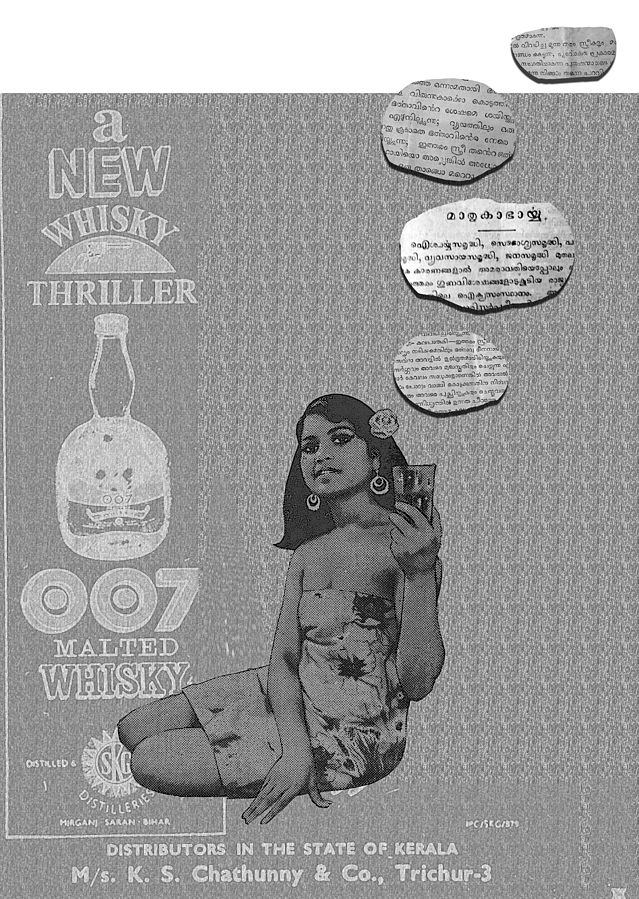
\includegraphics[width=0.7\textwidth,height=8cm]{Kulasthree_Chapter_four_pic03.jpg}
\end{center}
%\caption*{പുലയർ - കെ പി പത്മനാഭ മേനോൻ - വാള്യം 3, (1929), 1984}
\end{figure}



\captionof{mybox}{മലയാളിസ്ത്രീകളുടെ തൊഴിൽപങ്കാളിത്തം}\label{ch4box1} % place the caption
\begin{tcolorbox}[%
 breakable, % make the box breakable
  arc=0mm, 
  left=1pt, right = 1pt, 
  boxrule=0mm,
  colback = {blue!10}, % since shadow-gray was not defined
] 

\begin{center}
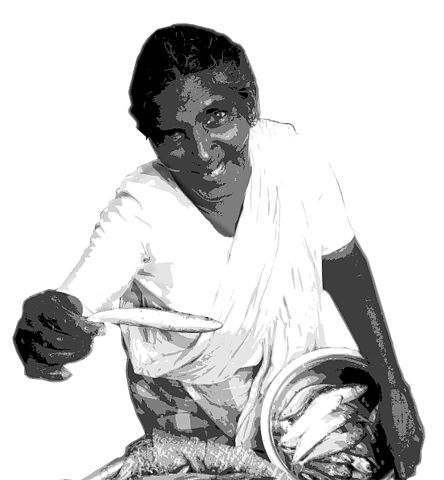
\includegraphics[width=0.4\textwidth,height=4cm]{Kulasthree_Chapter_four_pic04.jpg}
\end{center}
ഇരുപതാംനൂറ്റാണ്ടിൽ മലയാളിസ്ത്രീകളുടെ തൊഴിൽപങ്കാളിത്തനിരക്കിൽ ഗണ്യമായ ഇടിവുണ്ടായിട്ടുണ്ടെന്ന് സാമൂഹ്യശാസ്ത്രജ്ഞർ ചൂണ്ടിക്കാണിക്കുന്നു. 1901 മുതൽ 2011വരെയുള്ള കണക്കുകളാണ് താഴെ. പുരുഷന്മാരും സ്ത്രീകളും തമ്മിലുള്ള വിടവും വർദ്ധിച്ചുവെന്നു കാണാം. 

\begin{tabular}{ l c c r }
വർഷം &	പുരുഷൻ	& സ്ത്രീ &	വിടവ് \\
\hline
1901 &	56.3	&  32.7&	23.6\\
1911	& 53.8	& 28.9	& 24.9\\
1921&	51.1&	24.5&	26.6\\
1931	&50.0&	35.9&	14.1\\
1941&	ലഭ്യമല്ല&	ലഭ്യമല്ല	&ലഭ്യമല്ല\\
1951&	46.7&	18.3	&28.4\\
1961	&47.2	&19.7&	27.5\\
1971&	45.2	&14.6&	30.6\\
1981&	44.9&	16.6&	28.3\\
1991&	47.6&	15.9&	31.7\\
2001&	50.4	&15.3&	35.7\\
\end{tabular}

(S. Irudaya Rajan, Sreerupa, "Gender Disparity in Kerala : A Critical Reinterpretation', Swapna Mukhopadhyay (ed), The Enigma of the Kerala Woman, New Delhi, 2007, പുറം. 46)
\\
1931ൽ സ്ത്രീകൾ കൂടുതലായി തൊഴിൽരംഗത്തു പ്രവേശിച്ചതായി കാണുന്നുവെങ്കിലും 1951ൽ അവരുടെ തൊഴിൽപങ്കാളിത്തനിരക്ക് തീരെ കുറഞ്ഞതായി കാണുന്നു. പിന്നീട് ഏറെക്കുറെ താഴേക്കുതന്നെയാണാ അതിന്റെ പോക്ക്. എന്നാൽ 1931ലെ വർദ്ധനവ് സെൻസസ് വിവരശേഖരണരീതിയിൽ ആ തവണ ഉണ്ടായ മാറ്റംകൊണ്ടാകാം.
\end{tcolorbox}



\paragraph{}ജോസഫ് മൂളിയിൽ രചിച്ച സുകുമാരി (1897) എന്ന നോവലിൽ ജാതിവ്യത്യാസത്തെയും അസമത്വത്തെയും ന്യായീകരിച്ച ജാതിക്രമവും ആൺ-പെൺ വ്യത്യാസത്തിലൂന്നിയ ലിംഗക്രമവും തമ്മിൽ നേർക്കുനേർ ഇടയുന്ന ഒരു സന്ദർഭമുണ്ട്. കീഴ്ജാതിയിൽനിന്ന് ക്രിസ്തുമതം സ്വീകരിച്ച ഒരുവനാണ് ലിംഗക്രമത്തിന്റെ വക്താവായി നോവലിൽ പ്രത്യക്ഷപ്പെടുന്നത്. ഇതു കീഴ്ജാതികൾക്ക് നൽകിയ ആത്മവിശ്വാസം ശ്രദ്ധേയമാണ്.

\begin{quotation}
\noindent ശ്രീചിത്തിരതിരുന്നാൾ തിരുമനസ്സിലേക്ക് പ്രായപൂർത്തിയാകുംവരെ ആറ്റിങ്ങൽ മൂത്തതമ്പുരാൻ തിരുമനസ്സുകൊണ്ട് ഭരണാധികാരിയായിരിക്കുന്നതാണ്. അവിടത്തെ അധികാരം അവിഭാജ്യമായിക്കാണണമെന്നും ആകുന്നു ഈ രാജ്യത്തെ ഭൂരിപക്ഷം ആളുകളുടെയും അഭിപ്രായം. ഈ അഭിപ്രായം കീഴ്‌നടപ്പിനും മരുമക്കത്തായ നിയമത്തിനും അനുസരണമായിത്തന്നെ ഇരിക്കുന്നു. മരുമക്കത്തായ നിയമപ്രകാരം പ്രായപൂർത്തിയായ പുരുഷന്മാരുണ്ടെങ്കിൽ അവർ കുടുംബഭരണം നടത്തുന്നതും അവരുടെ അഭാവത്തിൽ വയസ്സ് മൂപ്പുളള സ്ത്രീ കാരണവത്തിയായിരിക്കുന്നതുമാണ്. കാരണവത്തി കുടുംബഭരണം നടത്തുന്നത് ഭാവിയിൽ കാരണവൻ ആകുന്ന പുരുഷന്റെ പ്രതിനിധിയെന്ന നിലയിലല്ല. കുടുംബത്തിലെ മൂത്തയാൾ എന്ന നിലയിലാണ്. ഇങ്ങനെ വയസ്സുമൂപ്പുളള സ്ത്രീ കാരണവത്തിയായിരിക്കുന്നിടേത്താളംകാലം സ്വന്തംനിലയിൽത്തന്നെ ഭരണാധികാരിയായിരിക്കുന്നതുമാണ്. ഹിന്ദുനിയമപ്രകാരമുളള അവകാശക്രമം ഇതിൽനിന്ന് വ്യത്യസ്തമായിരിക്കുന്നു. [അതിൽ] സ്ത്രീകൾ ഭരണം നടത്തുന്നുവെങ്കിൽ, പുരുഷന്മാരുടെ പ്രതിനിധികളെന്ന നിലയിലാണ്. വാസ്തവത്തിൽ മരുമക്കത്തായമനുസരിച്ച് സ്ത്രീകൾ കുറച്ചുകാലത്തേക്കുമാത്രം കാരണവത്തികളായിരുന്നാലും അവർ ഭരണംനടത്തുന്നത് സ്വാധികാരമനുസരിച്ചാണെന്നതിന് സംശയമില്ല.
\flushright{(ജോസഫ് മൂളിയിൽ, സുകുമാരി, ജോർജ് ഇരുമ്പയം (സമ്പാ.), നാലു നോവലുകൾ, തൃശൂർ, (1897), 1985, പുറം. 362)}
\end{quotation}

എത്രതന്നെ 'സ്വാഭാവിക'മായി അനുഭവപ്പെട്ടാലും, ഈ വിശ്വാസത്തിൽനിന്ന് നമ്മുടെ സമൂഹം - എന്തിന്, ലോകംമുഴുവൻ - വളരെയധികം മുന്നോട്ടുപോയിക്കഴിഞ്ഞിരിക്കുന്നുവെന്ന വസ്തുത ഇവിടെ പ്രത്യേകം എടുത്തുപറയേണ്ടതാണ്. സ്ത്രീകളുടെ 'സ്ത്രീത്വം', പുരുഷന്മാരുടെ 'പുരുഷത്വം' മുതലായവയെ പ്രകൃതിനിർണ്ണിതഗുണങ്ങളായി കാണാനാവില്ലെന്ന് നാം ഇന്നറിയുന്നു. ഒരിക്കലും മാറാത്തവിധം 'ആൺ'-'പെൺ' സ്വഭാവങ്ങൾക്ക് ദൃഢത നൽകുന്ന യാതൊന്നും പ്രകൃതിയിലില്ലെന്ന് ശാസ്ത്രഗവേഷണം വെളിപ്പെടുത്തുന്നു. ഈ സ്വഭാവങ്ങൾ സാമൂഹ്യജീവിതത്തിന്റെ ഭാഗമായി സൃഷ്ടിക്കപ്പെടുന്നവയാണെന്നും സാമൂഹ്യമാറ്റത്തിലൂടെ അവയും മാറ്റത്തിനു വിധേയമാകുന്നുവെന്നും പരക്കെ സമ്മതിക്കപ്പെടുന്നു. ലിംഗവ്യത്യാസത്തെ ഒന്നുകിൽ 'ആൺ' അല്ലെങ്കിൽ 'പെൺ' എന്നു വേർതിരിച്ചുകണ്ടിരുന്ന രീതിതന്നെ അപ്രസക്തം, അല്ലെങ്കിൽ അനുചിതമായിമാറുന്ന ഒരു ലോകമാണ് ഇന്ന്. പുരുഷശരീരത്തോടെ ജനിച്ചാലും സ്ത്രീയായി ജീവിക്കാനാഗ്രഹിക്കുന്നവർ, സ്ത്രീശരീരമാണെങ്കിലും പുരുഷനാണെന്നുതന്നെ വിശ്വസിക്കുന്നവർ, സ്വവർഗ്ഗസ്നേഹികൾ - ഇങ്ങനെ ലിംഗഭേദത്തെ വളരെ വ്യത്യസ്തമായ രീതികളിൽ വീക്ഷിക്കുന്നവർ ക്രമേണ പൊതുസമൂഹത്തിന്റെ ഭാഗമായിക്കൊണ്ടിരിക്കുന്നു. കഠിനമായി പീഡിപ്പിക്കപ്പെട്ടവരാണിവർ - 'പ്രകൃതിവിരുദ്ധർ' എന്ന പേരിൽ. എന്നാലിന്ന് അവരുടെ താൽപര്യങ്ങളിലും പെരുമാറ്റത്തിലും 'പ്രകൃതിവിരുദ്ധ'മായി യാതൊന്നുമില്ല എന്നു കരുതുന്ന വലിയൊരു വിഭാഗമുണ്ട്. സംഘടിതമതങ്ങളും മതമേധാവികളും ഇവരെ അംഗീകരിക്കാൻ തയ്യാറല്ലെങ്കിലും മതത്തിനുപുറത്ത് അവർ അംഗീകരിക്കപ്പെടുന്നു. പൊതുവെ ലിംഗപ്രത്യേകതകൾ പ്രകൃതിയോ ദൈവമോ നിർണ്ണയിക്കുന്നവയാണെന്ന വിശ്വാസത്തിന് മതവിശ്വാസത്തിന്റെ ഉന്നതവൃത്തങ്ങൾക്കുപുറത്ത് പണ്ടത്തെയത്ര ശക്തിയില്ല. സ്ത്രീകൾ വീട്ടുകാരികളായിരിക്കണമെന്ന് പ്രകൃതിനിയമമൊന്നുമില്ലെന്ന് സുവ്യക്തമാണ്. സമൂഹത്തിലെ മറ്റു സ്വാധീനങ്ങളുടെ പ്രാധാന്യം അംഗീകരിക്കപ്പെടുന്നുമുണ്ട്.

\begin{figure}[h]
\begin{center}
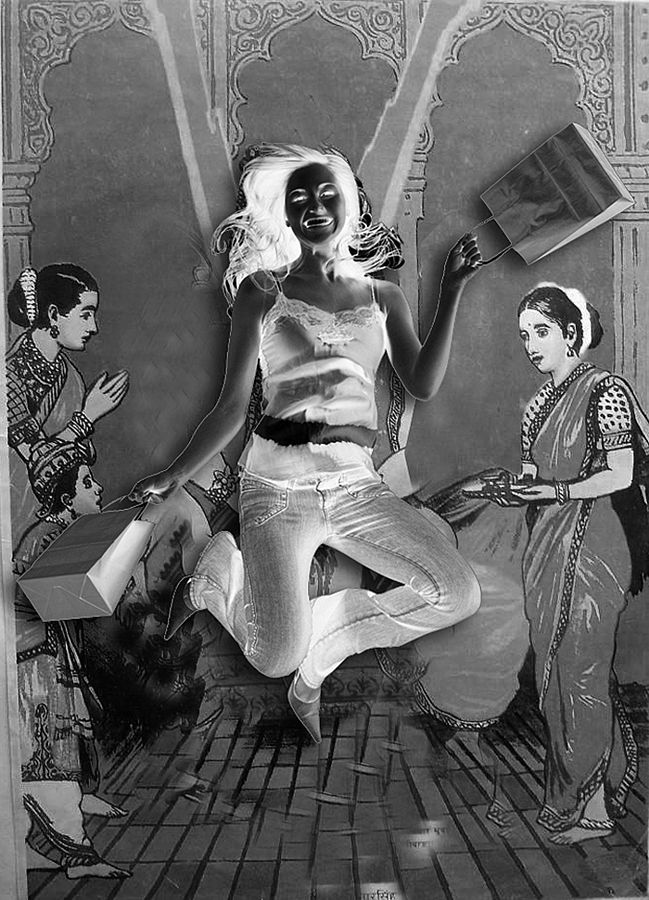
\includegraphics[width=0.7\textwidth,height=8cm]{Kulasthree_Chapter_four_pic05.jpg}
\end{center}
%\caption*{പുലയർ - കെ പി പത്മനാഭ മേനോൻ - വാള്യം 3, (1929), 1984}
\end{figure}


\paragraph{}പക്ഷേ, 19-ാം നൂറ്റാണ്ടിലും 20-ാം നൂറ്റാണ്ടിലുമുള്ള നവവരേണ്യചിന്തയെ ലിംഗഭേദത്തിന്റേതായ ഈ പരിപ്രേക്ഷ്യം ആഴത്തിൽ സ്വാധീനിച്ചു. സ്ത്രീകളുടെയും പുരുഷന്മാരുടെയും മാന്യതയെക്കുറിച്ചുള്ള പുതിയ ധാരണകളെ രൂപപ്പെടുത്തുന്നതിൽ ഇതിനു മുഖ്യപങ്കുണ്ടായിരുന്നു. വ്യത്യസ്ത ജാതികളിൽപ്പെട്ട സ്ത്രീകൾക്ക് വളരെ വ്യത്യസ്തങ്ങളായ ലിംഗാദർശങ്ങൾ ബാധകമായിരുന്നുവെന്ന് മുമ്പൊരു അദ്ധ്യായത്തിൽ വിവരിച്ചുവല്ലോ. ഇതിനു ബദലായിവന്ന പുതിയ സാമൂഹികാദർശമാതൃകയിൽ എല്ലാ സ്ത്രീകൾക്കും ഒരുപോലെ ബാധകമായ സ്ത്രീത്വാദർശമുണ്ടായിരുന്നു. 1913ൽ ഒരു സ്ത്രീസമാജത്തിൽ തച്ചാട്ടുദേവകിയമ്മ ചെയ്ത പ്രസംഗത്തിൽ ഈ ആദർശത്തെക്കുറിച്ച് വ്യക്തമായി വിവരിച്ചു പറയുന്നു:

\begin{quotation}

\noindent
സ്ത്രീകൾക്കും പുരുഷന്മാർക്കും ഒരേതരം വിദ്യാഭ്യാസം നൽകുന്നത് ആശാസ്യമല്ല. പ്രകൃതി ഇരുകൂട്ടരേയും ഒരേ ധർമ്മത്തിനല്ല സൃഷ്ടിച്ചതെന്ന് അവരുടെ ശരീരം, മാനസികാവസ്ഥ, ബുദ്ധിപരമായ കഴിവുകൾ എന്നിവയിൽനിന്നു തെളിയുന്നുണ്ട്... സ്ത്രീയുടെ ശരീരസ്ഥിതിയും മനഃസ്ഥിതിയും പരിശോധിച്ചാൽ, കൂടുതൽ ശരീരശക്തി വേണ്ടാത്ത, എന്നാൽ അധികം സഹനശേഷി ആവശ്യമുള്ള പ്രവൃത്തികൾക്കായാണ് അവൾ സൃഷ്ടിക്കപ്പെട്ടതെന്ന് തീർച്ചയാണ്. പ്രായേണ സ്ത്രീയുടെ മനോഘടന കോമളവും, വേഗത്തിൽ പരിപക്വമാവുന്നതും, ഭാവനാപൂർണ്ണവും, വികാരങ്ങൾക്കു വേഗം അടിപ്പെടുന്നതും, സൂക്ഷ്മസ്ഥിതികളെ ഗ്രഹിക്കുന്നതും, വേഗം ഇളകുന്നതുമാണ്. ദയ, സ്നേഹം, ക്ഷമ മുതലായ ഗുണങ്ങളിൽ പുരുഷൻ സ്ത്രീയുടെ സമീപത്ത് ഒരിക്കലും എത്തുകയില്ല...

\noindent
സ്ത്രീകൾ പൊതുരംഗത്തു പ്രവേശിച്ചില്ലെങ്കിലും അവർ കഴിവുള്ള സന്തതികളെ വളർത്തിയാൽ, അതുതന്നെ ലോകക്ഷേമത്തിനവർ നൽകുന്ന സംഭാവനയല്ലയോ? അതുകൊണ്ട് അവരുടെ വിദ്യാഭ്യാസത്തിന്റെ ലക്ഷ്യം അവരെ രണ്ടാംകിട പുരുഷന്മാരാക്കലല്ല, മറിച്ച് ദയ, കരുണ, സ്നേഹം, മമത, ക്ഷമ മുതലായ ഗുണങ്ങളെ വളർത്തലാണ്... ജീവിതസമരത്തിൽ പുരുഷന്റെ സഹായിയായി, തന്റെ സ്ത്രീത്വത്തിലൂടെ അവന്റെ അദ്ധ്വാനത്തെ ലഘൂകരിക്കലാണ് സ്ത്രീയുടെ ധർമ്മം. ദയാപൂർണ്ണമായ വാക്കിലൂടെയും പ്രവൃത്തിയിലൂടെയുമാണ് സ്ത്രീ വിജയംവരിക്കേണ്ടത്. മത്സരത്തിലൂടെയല്ല...

\flushright{(തച്ചാട്ട് ദേവകി അമ്മ, 'സ്ത്രീവിദ്യാഭ്യാസത്തിന്റെ ഉദ്ദേശം', ലക്ഷ്മീഭായി 20(1),1913-14)}
\end{quotation}

\paragraph{}
 'ശരീരശക്തി' സ്ത്രീക്കു കുറവാണെന്ന് ദേവകിയമ്മ പറയുന്നുണ്ടെങ്കിലും കഠിനമായ കായികജോലികളിൽ അക്കാലത്തെ സ്ത്രീകൾ ഏർപ്പെട്ടിരുന്നതിനെക്കുറിച്ച് മുൻ അദ്ധ്യായത്തിൽ പറഞ്ഞുവല്ലോ. അതിൽ വിവരിച്ചതിലധികം ശ്രമകരമായ ജോലികൾ ചെയ്തിരുന്ന ദരിദ്രസ്ത്രീകൾ ഈ നാട്ടിൽ ധാരാളമുണ്ടായിരുന്നു. തിരുവനന്തപുരത്തെ ചാലക്കമ്പോളത്തിൽ ചുമടെടുത്ത് കഴിഞ്ഞിരുന്ന സ്ത്രീകൾ അക്കാലത്തുണ്ടായിരുന്നു. വിദൂരസ്ഥലങ്ങളിൽനിന്ന് വലിയ ചാക്കുകളിൽ നെല്ലുചുമന്ന് ചാലയിലെത്തി വിൽപന നടത്തിയിരുന്ന സ്ത്രീകളുണ്ടായിരുന്നു. തിരുവനന്തപുരത്തെ കിഴക്കൻ മലയോരപ്രദേശങ്ങളിൽനിന്ന് ഭാരമേറിയ പുൽക്കെട്ടുകൾ തലച്ചുമടായി വഹിച്ച് നഗരത്തിൽവന്ന് കച്ചവടം ചെയ്തിരുന്ന കീഴാളസ്ത്രീകൾക്ക്, പക്ഷേ, ആ ചുമട് നിലത്തുവച്ചു കച്ചവടം ചെയ്യാൻ അനുമതിയില്ലായിരുന്നു. ഇതിനെതിരെ ശ്രീമൂലം പ്രജാസഭയിൽ അധഃസ്ഥിതരുടെ പ്രതിനിധിയും തിരുവിതാംകൂറിലെ കീഴാളരുടെ നേതാവും ഗുരുവുമായിരുന്ന പൊയ്കയിൽ അപ്പച്ചൻ (യോഹന്നാൻ) 1930കളിൽ ശബ്ദമുയർത്തിയതിനെത്തുടർന്നാണ് പുൽക്കെട്ടു നിലത്തിറക്കിവച്ചു കച്ചവടം ചെയ്യാനുള്ള അനുമതി കീഴാളസ്ത്രീകൾക്കു ലഭിച്ചത്. (കാണുക \ref{ch2box7})	പുരുഷന്റെയൊപ്പം പേശീബലമില്ലെങ്കിലും കായികമായ സഹനശക്തി, തീർച്ചയായും ഈ സ്ത്രീകളിൽ കുറവായിരുന്നില്ല. അവർക്ക് ശരീരശക്തി കുറവായിരുന്നുവെന്നു പറയാനും എളുപ്പമല്ല - നെൽച്ചാക്കും തലയിൽവഹിച്ച് അനേകം കാതം നടന്ന് ചന്തയിൽ പോകാൻ ശരീരശക്തികൂടാതെ പറ്റില്ലല്ലോ. എന്തായാലും വെയിലേറ്റ ചീരത്തണ്ടുപോലെ വാടിക്കുഴയുന്ന ദേഹമല്ലായിരുന്നിരിക്കണം, ഇവരുടേത്! ദേവകിയമ്മയുടെ സ്ത്രീത്വാദർശം മേലാളമൂല്യങ്ങളിൽ പങ്കുചേരുന്നവയാണ് എന്ന് നിസ്സംശയം പറയാം. ദേഹാദ്ധ്വാനംകൊണ്ടു ജീവിക്കുന്ന സ്ത്രീകൾ, കായികശേഷി പ്രകടിപ്പിക്കുന്ന സ്ത്രീകൾ - ഇവരെല്ലാം ദേവകിയമ്മയുടെ സ്ത്രീത്വാദർശത്തിനു പുറത്താണ്! ഇതേകാലത്തുതന്നെ സ്ത്രീകൾക്കു പുരുഷന്മാരെപ്പോലെ സാമൂഹ്യജീവിതത്തിലും പൊതുരംഗത്തും ഇറങ്ങി പ്രവർത്തിക്കാൻ കഴിവുണ്ടെന്നു വാദിച്ച മറ്റു ലേഖകരുമുണ്ടായിരുന്നു - എന്നാൽ അവരും 'സ്ത്രീത്വ'ത്തിന്റെ സവിശേഷതയ്ക്ക്, വ്യവസ്ഥയ്ക്ക്, പ്രത്യേകമൂന്നൽ നൽകുകതന്നെ ചെയ്തു.

\paragraph{}'ദയ, സ്നേഹം, ക്ഷമ' - ഇവയൊക്കെ സ്ത്രീസഹജഗുണങ്ങളാണെന്നാണ് ദേവകിയമ്മയും മറ്റുപലരുമെഴുതിയത്. വികാരങ്ങൾ - പ്രത്യേകിച്ച് മൃദുലവികാരങ്ങൾ - പൊതുവെ സ്ത്രീയുടെ സഹജവാസനയെ നിർണ്ണയിക്കുന്നുവെന്നു പറയുന്നതുകൊണ്ടുള്ള പരോക്ഷഫലമെന്താണ്? പൊതുവെ യുക്തിയുടെ ലോകത്തെ ഒന്നടങ്കം പുരുഷന്മാർക്കു തീറെഴുതിക്കൊടുക്കുന്നതിനു സമമാണിത്! ഇന്ന് കേരളത്തിലെ ബൗദ്ധികജീവിതത്തിൽ നാം കാണുന്ന ചില പ്രത്യേകതകളുടെ വേരുകൾ ഇത്തരം ധാരണകളിലല്ലേ എന്നു സംശയിച്ചുപോകുന്നു. പൊതുവെ സാഹിത്യം വികാരങ്ങളുടെ ഉൽപന്നമായാണ് കണക്കാക്കപ്പെടുന്നത് - കേരളത്തിലെ എഴുത്തികാരികളിലധികംപേരും സാഹിത്യരംഗത്താണ് നിലയുറപ്പിച്ചിട്ടുള്ളത്. സാഹിത്യേതരരംഗങ്ങളിൽ സ്ത്രീകൾ പൊതുവെ കുറവാണ്: നിരൂപണം, ശാസ്ത്രം, സാമൂഹ്യശാസ്ത്രം ഇതെല്ലാം പുരുഷന്മാരുടെ മേഖലകളാണ്. പൊതുവെ യുക്തി, ലോകപരിചയം, ഇവ ആവശ്യപ്പെടുന്ന ബൗദ്ധികപ്രവർത്തനങ്ങളിൽ ഏർപ്പെടുന്ന സ്ത്രീകളെ 'പൗരുഷക്കാരി'കളായി എണ്ണുന്ന സമൂഹമാണിത്.

\paragraph{}പുരുഷന്മാരുടേതായ പല മേഖലകളിലും കടന്നുചെല്ലാൻ 1920കൾക്കുശേഷം അഭ്യസ്തവിദ്യരായ സ്ത്രീകൾ ശക്തമായ ശ്രമങ്ങൾ ആരംഭിച്ചുവെങ്കിലും ആൺ-പെൺ വ്യത്യസ്തതയിലൂന്നിയ ഈ ലിംഗമാതൃകയെ അവർ കൈവെടിഞ്ഞില്ല. ആത്മനിയന്ത്രണത്തിലൂടെ സ്വന്തം കുടുംബത്തെ 'സൗമ്യമായ അധികാരത്തിലൂടെ' ഭരിക്കാൻ (അതായത്, സ്നേഹിച്ചും ശാസിച്ചും നേർവഴി നടത്തിക്കാനുള്ള അധികാരത്തിലൂടെ - ശിക്ഷിച്ചും താഡിച്ചും ഭരിക്കാനുള്ള അധികാരത്തിൽനിന്ന് ഇത് വ്യത്യസ്തമാണ്) സവിശേഷമായ കഴിവാണല്ലൊ പുതിയ സ്ത്രീദർശനം സ്ത്രീക്കു കൽപ്പിച്ചത്. ഈ കഴിവ് കുടുംബത്തിനുപുറത്തും ഏറ്റവും പ്രസക്തമാണെന്ന് അഭ്യസ്തവിദ്യരായ ഈ സ്ത്രീകൾ - കേരളീയ സ്ത്രീവാദികളുടെ ആദ്യതലമുറ - വാദിച്ചു. അതായത് വീട്ടിൽ മാത്രമല്ല, പൊതുസ്ഥാപനങ്ങളിലും (വിദ്യാലയം, ആശുപത്രി, ഭരണസ്ഥാപനങ്ങൾ, കോടതികൾ, നിയമനിർമ്മാണസഭകൾ, ക്രമസമാധാനപാലന സ്ഥാപനങ്ങൾ) സ്ത്രീയുടെ 'സൗമ്യാധികാരം' ഫലപ്രദമായ ഭരണത്തിനുതകുമെന്നായിരുന്നു ഇവരുടെ അഭിപ്രായം. വിവാഹം കഴിക്കാതെയും പ്രസവിക്കാതെയും സ്ത്രീകൾക്ക് ഈ അധികാരം വിനിയോഗിക്കാമെന്ന സൂചന ഈ വാദത്തിലുണ്ടായിരുന്നുവെന്നത് ശ്രദ്ധേയമാണ്. പക്ഷേ, 'ആത്മനിയന്ത്രണ'ത്തിലൂടെ മാത്രമേ സ്ത്രീക്ക് തനിക്കു സഹജമെന്നു പറയപ്പെട്ട 'സൗമ്യാധികാര'ത്തെ പുറത്തെടുക്കാനാവൂ. അതുകൊണ്ടുതന്നെ, തന്റെമേൽ കടുത്ത നിയന്ത്രണങ്ങൾ സ്വയമേൽക്കുന്ന സ്ത്രീ മാത്രമേ ഉത്തമസ്ത്രീയാകൂ എന്ന ധാരണയെ കുറച്ചുകൂടി ഉറപ്പിക്കാൻ ആദ്യകാല സ്ത്രീവാദികളുടെ മേൽവിവരിച്ച അവകാശവാദം സഹായിച്ചു. 'സ്ത്രീയുടെ സഹജമായ കഴിവാ'ണിതെന്നമട്ടിലാണ് ആദ്യകാല സ്ത്രീവാദികളും ഇതിനെ അവതരിപ്പിച്ചത്. 1916ൽ 'സരോജിനി' എന്ന തൂലികാനാമത്തിൽ പ്രത്യക്ഷപ്പെട്ട ലേഖനത്തിൽ ഈ തന്ത്രം പ്രവർത്തിക്കുന്നതു കാണാം.





\captionof{mybox}{മതസമൂഹങ്ങളും സ്ത്രീകളും}\label{ch4box2} % place the caption
\begin{tcolorbox}[%
 breakable, % make the box breakable
  arc=0mm, 
  left=1pt, right = 1pt, 
  boxrule=0mm,
  colback = {blue!10}, % since shadow-gray was not defined
] 
\paragraph{}
\begin{center}
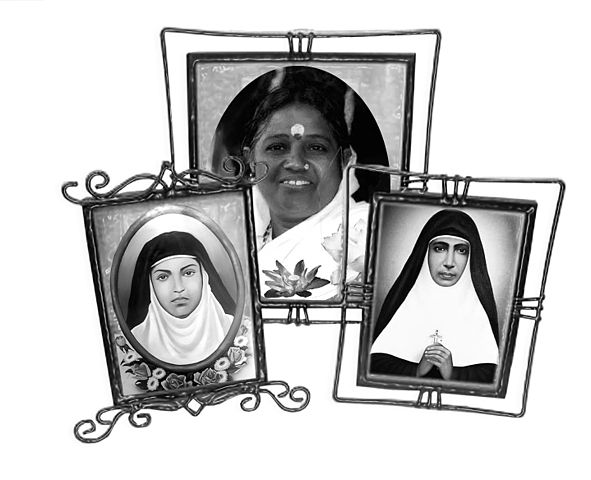
\includegraphics[width=0.4\textwidth,height=4cm]{Kulasthree_Chapter_four_pic06.jpg}
\end{center}

സമുദായങ്ങളെ കൂടുതൽ ജനാധിപത്യവൽക്കരിക്കണം; സ്ത്രീകൾക്ക് സമുദായങ്ങൾക്കുള്ളിൽ നീതിയും സംരക്ഷണവും തുല്യതയും ലഭിക്കണം - ഇത്തരം മുദ്രാവാക്യങ്ങൾ ഉന്നയിച്ചുകൊണ്ടാണ് സമുദായപരിഷ്ക്കർത്താക്കളായ സ്ത്രീകൾ രംഗപ്രവേശം ചെയ്തത്. എന്നാൽ മതവിശ്വാസത്തിനുള്ളിൽ ഇത്തരമൊരു ലിംഗജനാധിപത്യത്തിനുവേണ്ടി വാദങ്ങളുണ്ടായി എന്നു പറയാനാവില്ല. സ്ത്രീകൾക്ക് തീരെ ആനുകൂല്യം ലഭ്യമല്ലായിരുന്ന ഈ രംഗത്ത് - അസാമാന്യമായ സാന്നിദ്ധ്യവും വമ്പിച്ച നേട്ടവും കൈവരിച്ച ഒന്നുരണ്ടു സ്ത്രീകൾ ഉണ്ടായിട്ടുണ്ടെന്നു തീർച്ച. അടുത്തിടെ മാർപ്പാപ്പ വിശുദ്ധയായി പ്രഖ്യാപിച്ച ഭരണങ്ങാനത്തെ അൽഫോൺസാമ്മ (1910-1946), വാഴ്ത്തപ്പെട്ട മറിയം ത്രേസ്യാമ്മ (1876-1926) എന്നിവരുടെ പേരുകൾ എടുത്തുപറയേണ്ടവയാണ്. സാമൂഹ്യപരിഷ്ക്കരണത്തിന്റെ അന്തഃസത്തയെ ക്രിസ്തീയസന്ന്യാസിനിമാരുടെ ജീവിതചര്യയുടെ ഭാഗമാക്കിയ മറിയം ത്രേസ്യ തൃശൂരിലെ പുത്തൻചിറയിൽ ജനിച്ചു. തിരുകുടുംബ സന്യാസിനീസഭ (Congregation of the Holy Family) എന്ന സംഘം സ്ഥാപിക്കുന്നതിലൂടെ അവർ സേവനത്തെ സന്യാസജീവിതത്തിന്റെ ഭാഗമാക്കി. 20-ാം നൂറ്റാണ്ടിൽ കത്തോലിക്കാസഭയിൽ സന്യാസിനിമാരുടെ എണ്ണം ഗണ്യമായി വർദ്ധിച്ചു - 1960കൾക്കും 1970കൾക്കുമിടയിൽ സന്യാസിനികളായി ചേർന്നവരുടെ എണ്ണം വർഷത്തിൽ ഇരുപതു ശതമാനംവച്ചു വർദ്ധിച്ചുവെന്ന് Genevieve Lemercinier, F.Houtart എന്നിവരുടെ പഠനം വെളിപ്പെടുത്തുന്നു. (The Church and Development in Kerala, കൊച്ചി, 1974). എന്നാൽ ഇതനുസരിച്ച് സന്യാസിനിമാരുടെ അധികാരങ്ങളിൽ മാറ്റമുണ്ടായി എന്നു കരുതാനാവില്ല.

\paragraph{}

ആത്മീയപ്രവർത്തനങ്ങളിലെ സ്ത്രീപങ്കാളിത്തം ഇനിയുമേറെ പഠനങ്ങൾ നടക്കേണ്ട വിഷയമാണ്. കേരളത്തിലെ ഹിന്ദുമതവിശ്വാസത്തിന്റെ സമീപകാലചരിത്രത്തിൽ ഉന്നതജാതിക്കാരായ പുരുഷന്മാർക്കു സന്യാസദീക്ഷ നൽകുന്ന [കീഴ്ജാതിയിൽ പിറന്ന] ആത്മീയനേതാവായ സ്ത്രീ എന്ന നിലയിൽ മാതാ അമൃതാനന്ദമയി വളരെ പ്രധാനപ്പെട്ട ഒരു പ്രതിഭാസമാണ്. എന്നാൽ വിശ്വാസത്തിന്റെ രംഗത്ത് അവർക്ക് മുൻഗാമികളുണ്ടായിരുന്നു - അവരെക്കുറിച്ച് നമുക്കധികമൊന്നും അറിയില്ലെങ്കിലും. മാസമുറയുള്ള കാലത്ത് സ്ത്രീകൾ ദേവാലയങ്ങളിൽ പ്രവേശിച്ചുകൂടെന്ന വിലക്ക് തികച്ചും മതപരമാണ്. ഈ വിലക്കിന്റെ സ്ത്രീവിരുദ്ധതയെ ചോദ്യംചെയ്യുന്ന ശബ്ദങ്ങൾ മതങ്ങൾക്കുള്ളിൽ തീരെ കേൾക്കാനില്ല - സ്ത്രീകളായ വിശ്വാസികളുടെ എണ്ണം വളരെവളരെ വലുതായ ഇക്കാലത്തും.
\end{tcolorbox}

ലൈംഗികമായ അച്ചടക്കം - അതായത് ഒരേയൊരു ഭർത്താവ് മാത്രമുണ്ടാവുക, ഭർത്താവിന്റെ ഹിതമനുസരിച്ച് ജീവിക്കുക, അദ്ദേഹത്തിനോട് ലൈംഗികമായ വിശ്വസ്തത പുലർത്തുക - ഇതൊക്കെ 'സ്ത്രീസഹജ'മാണെന്നായിരുന്നു അവരുടെ അഭിപ്രായം:
\begin{quotation}

\noindent

സീത രാവണാലയത്തിൽ ഒരാണ്ടു പാർത്ത സംശയം പോക്കാൻ തീയിൽ ചാടിയിട്ടും ശ്രീരാമനും മാലോകർക്കും സംശയം നീങ്ങിയില്ല. ലക്ഷ്മണൻ പന്തീരാണ്ടുകാലം തന്നെപ്പിരിഞ്ഞു പാർത്തിട്ടും കള്ളുകുടിച്ച തണ്ടാൻ തെങ്ങിൽ കയറിയമാതിരി ശൂർപ്പണഖയുടെ മൂക്കിലുംമറ്റും പാഞ്ഞിട്ടും ഊർമ്മിളയ്ക്കു ഒരു സംശയവുമുണ്ടായില്ല. വേശ്യാഗൃഹത്തിൽ പോകണമെന്ന് ആവശ്യപ്പെട്ട കുഷ്ഠക്കാരനെ ശീലാവതി തോളിൽ ചുമന്നാണ് കൊണ്ടുപോയത്. വഴിക്കുവച്ചു മരിച്ചുപോയ ആ മഹാമൂർഖനെ തിര്യെ കൊടുത്തല്ലാതെ സൂര്യൻ ഉദിച്ചുകൂടെന്നു ശീലാവതി തറ്റുടുത്തുനിന്നുകൊണ്ടാണ് തപസ്സു ചെയ്തത്.

\noindent
....സ്ത്രീയെ കൊതിച്ച് പുരുഷന്മാർ പൊരുതി മരിച്ചതായി പുരാണങ്ങളും ചരിത്രങ്ങളുമുണ്ട്. പുരുഷന്മാർക്കുവേണ്ടി സ്ത്രീകൾ വാക്കേറ്റംപോലും നടത്തിയതായി പുരാണവുമില്ല, ചരിത്രവുമില്ല... അതാണ് സ്ത്രീത്വം.
\flushright{(സരോജിനി, 'സ്ത്രീത്വം', മഹിളാരത്നം 1 (5), 1916)}
\end{quotation}

\paragraph{}
ഈ ഒടുവിലത്തെ പ്രസ്താവം വസ്തുതാപരമായി ശരിയല്ലെന്നു തീർച്ചയാണ് - പുരുഷന്മാരെച്ചൊല്ലി മല്ലടിച്ച സ്ത്രീ പുരാണത്തിലും ചരിത്രത്തിലുമുണ്ട്. ഒരുപക്ഷേ, പുരുഷന്മാരെപ്പോലെ അധികാരപദവിയില്ലാത്തതുകൊണ്ട് 'പൊരുതിമരിക്കാൻ' അവർക്കിടവന്നില്ലായിരിക്കാം! 'മാന്യസ്ത്രീ' - അതായത് 'സൗമ്യാധികാരം വഹിക്കാൻ പ്രാപ്തയായ സ്ത്രീ' - ലൈംഗികമായ ആഗ്രഹം ഒട്ടുമില്ലാത്തവളാണെന്നു വാദിക്കാനാണ് ലേഖിക തയ്യാറാവുന്നത്. വിദുഷിയായിരുന്ന ലേഖികയ്ക്ക് കൃഷ്ണന്റെ ഭാര്യമാർ തമ്മിലുള്ള പോരിനെക്കുറിച്ചും അർജ്ജുനപത്നിമാരുടെ വഴക്കിനെക്കുറിച്ചും കൈകേയിയുടെ സാമർത്ഥ്യത്തെപ്പറ്റിയും ഉർവ്വശിക്ക് അർജ്ജുനനനോടു തോന്നിയ കാമത്തെക്കുറിച്ചും അറിയില്ലായിരുന്നുവെന്ന് കരുതാൻ ന്യായമില്ലല്ലോ! സ്ത്രീകളുടെമേൽ ഇരട്ടസദാചാരം വച്ചുകെട്ടുന്ന രീതിയെ അപലപിക്കാനാണ് അവർ ശ്രമിച്ചത്; പക്ഷേ, അതിനിടയിലൂടെ അനാവശ്യമായ സദാചാരഭാരത്തെ സ്ത്രീയുടെ തലയിൽവച്ചുകെട്ടുകകൂടി ചെയ്യുന്നുമുണ്ട്.

\paragraph{}

അതേസമയം സ്ത്രീപുരുഷവ്യത്യാസം പരസ്പരപൂരകത്വത്തിലേക്കു നയിക്കണമെങ്കിൽ പുരുഷനും വളരെ പ്രധാനപ്പെട്ട ചുമതലകളുണ്ടെന്ന് ഓർമ്മപ്പെടുത്താൻ ആദ്യകാല സ്ത്രീവാദികൾ മറന്നില്ല. സ്ത്രീപുരുഷവ്യത്യാസത്തെ കൊണ്ടാടിയ ലേഖകരത്രയും സ്ത്രീപുരുഷപരസ്പരപൂരകത്വത്തിന്റെയും വക്താക്കളായിരുന്നു. അതായത് സ്ത്രീഗുണം, പുരുഷഗുണം എന്നിവ വ്യത്യസ്തങ്ങളാണെങ്കിലും അവയിലൊന്നുമാത്രമെ സാമൂഹ്യജീവിതത്തിൽ പ്രത്യക്ഷമാകുന്നുള്ളുവെങ്കിൽ ആ ജീവിതം അപൂർണ്ണമായിരിക്കുമെന്ന് അവർ കരുതി. സ്ത്രീപുരുഷന്മാർ പരസ്പരം ആശ്രയിച്ച്, പരസ്പരം ജീവിതത്തെ പൂർത്തീകരിച്ചുകൊണ്ട്, മുന്നേറണമെന്നായിരുന്നു ഇവരുടെ ആവശ്യം. ഇതിൽ സ്ത്രീയുടെ ചുമതലയെപ്പറ്റി ഘോരഘോരം പ്രസംഗിക്കുന്നവർ പുരുഷന്മാരുടെ ചുമതലയെക്കുറിച്ച് നിശ്ശബ്ദരാകുന്നുവെന്ന പരാതി ആദ്യകാല സ്ത്രീവാദികളിൽ പലരുമുന്നയിച്ചു. മിസിസ്സ് കെ. കണ്ണൻ മേനോൻ (ഇടത്തട്ട രുഗ്മിണിയമ്മയുടെ തൂലികാനാമങ്ങളിൽ ഒന്ന്) ഇതേക്കുറിച്ച് ഇങ്ങനെയെഴുതി:

\begin{quotation}

\noindent
തന്നെ ദേഹപ്രയത്നംകൊണ്ടു സംരക്ഷിച്ചും ഹൃദയപൂർവ്വം സ്നേഹിച്ചും വരുന്ന ഭർത്താക്കന്മാരെ ഭക്തിസ്നേഹബഹുമാനപുരസ്സരം ശുശ്രൂഷിച്ച്, അവരുടെ സൗകര്യം ശരിയായി നിർവ്വഹിക്കുന്നത് തങ്ങളുടെ ചുമതലയാണെന്നറിഞ്ഞ് ഏതുകാര്യത്തിന്നും സന്നദ്ധകളായിരിക്കുന്ന സ്ത്രീകൾ ഇപ്പോൾ ഒട്ടും ദുർലഭമല്ല. ഭർത്താവിന്റെ ആജ്ഞയ്ക്കനുസരിച്ച് നടക്കേണമെന്നും, അദ്ദേഹത്തെ സ്നേഹിക്കേണമെന്നും ഏതു സ്ത്രീക്കും ആരും ഉപദേശിക്കേണ്ട ആവശ്യമില്ല. ഇതു പ്രകൃതി സ്ത്രീഹൃദയത്തെ ആദ്യമായി പഠിപ്പിക്കുന്ന ഒരു പാഠമാണ്...

\noindent ഓരോ ബാലികയും തന്റെ യൗവ്വനാരംഭത്തോടുകൂടി ഒരു വരനെ ആഗ്രഹിച്ചുതുടങ്ങും. അവരവരുടെ ബുദ്ധിശക്തിയും സ്വഭാവഗുണങ്ങളും ആശ്രയിച്ചായിരിക്കും ഓരോരുത്തരും പുരുഷമാതൃകകളെ നിർമ്മിക്കുകയും, പിന്നീട് ഈ മാതൃകകളെ രൂപീകരിച്ച് ഭർത്താവിൽ കാണ്മാൻ ആഗ്രഹിക്കുകയും ചെയ്യുന്നത്. ഈ ആശയങ്ങളും ആഗ്രഹങ്ങളും സഫലമായാൽ ഒരു സ്ത്രീ 'ഭാര്യ' എന്ന പദവിയെ അർഹിക്കുകയും അതിന്റെ ചുമതലകൾ ശരിയായി നിറവേറ്റുകയും ചെയ്യുമെന്നു മാത്രമല്ല, വിഫലമായിത്തീരുന്നപക്ഷം ആ വിശിഷ്ടപദത്തെ മലിനപ്പെടുത്തുകയും ചെയ്യും.
\flushright{(മിസിസ്സ്. കെ. കണ്ണൻമേനോൻ, 'ആധുനിക വനിതാരത്നങ്ങളും അവരുടെ ഭർത്താക്കന്മാരും- ഒരു പ്രത്യാഖ്യാനം', മഹിളാരത്നം 1 (5), 1916)}
\end{quotation}

\paragraph{}ഉത്തമസ്ത്രീയുടെ ഇടം ഗൃഹമാണെന്ന വാദം സർവ്വത്ര കേട്ടുകൊണ്ടിരുന്ന സമയത്തുതന്നെ അവളുടെ കടമകളെക്കുറിച്ചുള്ള ധാരണകൾ മാറിക്കൊണ്ടിരുന്നു - സ്ത്രീക്ക് കൽപ്പിക്കപ്പെട്ട വീട്ടുത്തരവാദിത്തങ്ങളുടെ ഭാരം വർദ്ധിച്ചുകൊണ്ടിരുന്നു. 1920കൾക്കുശേഷം സാമ്പത്തികമാന്ദ്യമുണ്ടായത് ഇവിടത്തെ കൃഷിയെയും കച്ചവടത്തെയും കാര്യമായി ബാധിച്ചു; കൃഷിക്കാർ ബുദ്ധിമുട്ടിലായി. > കാണുക പുറം 105 < മരുമക്കത്തായ കൂട്ടുകുടുംബങ്ങൾ ഭാഗംവച്ചു പിരിയാൻ തുടങ്ങിയതോടുകൂടി രൂപപ്പെട്ട ചെറുകുടുംബങ്ങളിൽ പലതും വലിയ സാമ്പത്തിക വിഷമത്തിലകപ്പെട്ടു. ഈയവസരത്തിൽ ഗൃഹനായികയുടെ ജോലിയിൽ വീട്ടുഭരണവും ബാലപരിചരണവും മാത്രമല്ല, കുടുംബത്തിന്റെ സാമ്പത്തികഭാരം കുറയ്ക്കാനുള്ള പ്രവർത്തനവും ഉൾപ്പെടുമെന്ന വാദം ഉയർന്നുതുടങ്ങി. പരമ്പരാഗതകുടുംബങ്ങളിൽ സ്ത്രീകൾ നിർവ്വഹിച്ചിരുന്ന അതികഠിനമായ ഗാർഹിക ഉത്തരവാദിത്വങ്ങളെപ്പറ്റി കഴിഞ്ഞ അദ്ധ്യായത്തിൽ പറഞ്ഞല്ലൊ. ഈ ഭാരത്തിൽ ലേശവും കുറവുവരുത്തുന്ന യാതൊരു നടപടിയുമുണ്ടാവരുതെന്ന് പരിഷ്ക്കർത്താക്കൾക്ക് - അഭ്യസ്തവിദ്യകളായ സ്ത്രീകളുൾപ്പെടെയുള്ളവർക്ക് - നിർബന്ധമായിരുന്നു! അൽപ്പം സാമ്പത്തികസ്ഥിതി ആർജ്ജിച്ച കുടുംബങ്ങളിലെ സ്ത്രീകൾ വേലക്കാരെ നിയമിക്കുന്നുവെന്നുംമറ്റും ഇവർ ആരോപിച്ചു - തറവാട്ടുഭാഗം കഴിഞ്ഞുണ്ടായ അണുകുടുംബങ്ങളിൽ നേരിട്ടു വീട്ടുവേലയെടുക്കണമെന്നും, അതിനുപുറമെ ധനസമ്പാദനത്തിനുതകുന്ന തൊഴിലുകൾ വീട്ടിലിരുന്നു ചെയ്യണമെന്നും സ്ത്രീകളോടിവർ ആഹ്വാനം ചെയ്തു. കോന്നിയൂർ മീനാക്ഷിയമ്മ വാദിച്ചു:

\begin{quotation}
\noindent
പുതിയ  നായർ ബില്ലിന്റെ ആഗമനത്തോടുകൂടി ഓരോ വ്യക്തിക്കും സമുദായത്തിനു പൊതുവെയും ഉണ്ടായിട്ടുള്ള മുറിവിനെ കുടുംബഭരണപാടവംകൊണ്ടു സുഖപ്പെടുത്തേണ്ടത് നായർസ്ത്രീകളുടെ ഒഴിച്ചുകൂടാത്ത ധർമ്മമാകുന്നു...
ഭാഗപ്രകാരം കിട്ടുന്ന സ്വത്തിനെ അന്യാധീനപ്പെടുത്താതേയും നശിപ്പിക്കാതേയും സൂക്ഷിക്കേണ്ട വലുതായ ഭാരം സ്ത്രീകൾ വഹിക്കേണ്ടിയിരിക്കുന്നു... വീട്ടുവേലകൾ ചെയ്തശേഷമുള്ള സമയം വെറുതെ വെടിപറഞ്ഞുകളയാതെ മുറയ്ക്കു ധനസമ്പാദനത്തിനുതകുന്ന തൊഴിലുകൾ ചെയ്യുവാൻ വിനിയോഗിക്കണം.
\flushright{(കോന്നിയൂർ മീനാക്ഷിയമ്മ, 'നായർസ്ത്രീയും ഗൃഹവും' മഹിള 6(4), 1924)}
\end{quotation}

\begin{figure}[h]
\begin{center}
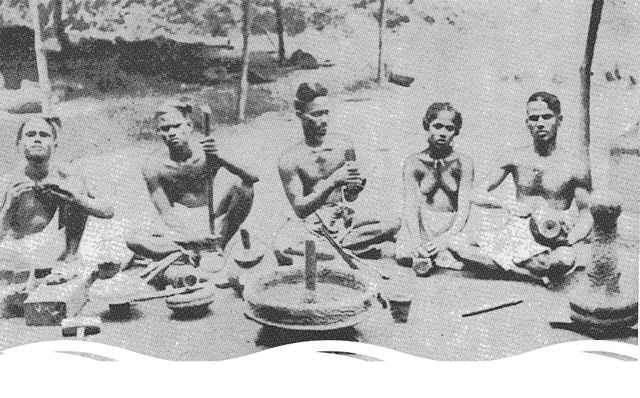
\includegraphics[width=\textwidth,height=8cm]{Kulasthree_Chapter_four_pic07.jpg}
\end{center}
%\caption*{പുലയർ - കെ പി പത്മനാഭ മേനോൻ - വാള്യം 3, (1929), 1984}
\end{figure}


\paragraph{}ചുരുക്കിപ്പറഞ്ഞാൽ, പുതിയ കുടുംബത്തിന്റെ അധിപ, 'ഗൃഹചക്രവർത്തിനി' എന്നുംമറ്റുമുള്ള വിശേഷണങ്ങൾ ആധുനികസ്ത്രീക്കു കൈവന്നെങ്കിലും രാപ്പകൽ വേലയെടുത്തില്ലെങ്കിൽ ആ പട്ടം നഷ്ടമായിപ്പോകുമെന്ന സ്ഥിതിയായിരുന്നു. എത്ര ദയനീയം! 'മാന്യസ്ത്രീകൾ' പക്ഷേ, വീട്ടിനകത്തിരുന്നേ ധനസമ്പാദനത്തിനു ശ്രമിക്കാവൂ എന്ന് ഇവരിൽ പലരും അനുശാസിക്കുന്നുണ്ട് (ഉദ്യോഗത്തിനിറങ്ങണമെന്നു വാദിച്ചവരുമുണ്ടായിരുന്നു - അത് മറ്റൊരദ്ധ്യായത്തിൽ). കൈവേലകൾ, തയ്യൽ, അടുക്കളത്തോട്ടം, കൃഷി, ഭക്ഷണവസ്തുക്കൾ തയ്യാറാക്കൽ - ഇത്തരം കുടിൽവ്യവസായങ്ങളാണ് സ്ത്രീകൾക്ക് ഉചിതമായി വിധിക്കപ്പെട്ടവ. പശുവളർത്തൽ മുതലായ ഗൃഹവ്യവസായപ്രവർത്തനങ്ങളിൽ ഏർപ്പെട്ടിരുന്ന സ്ത്രീകൾക്ക് സഹകരണസംഘംവഴി സഹായമെത്തിക്കണമെന്ന ആവശ്യം തിരുവിതാംകൂറിലെ നിയമനിർമ്മാണസഭയായിരുന്ന ശ്രീമൂലം പ്രജാസഭയിൽ സ്ത്രീകളെ പ്രതിനിധീകരിച്ച അംഗം പലതവണ ആവശ്യപ്പെട്ടു. സർക്കാർ സഹായത്തോടെ സഹകരണസംഘം രൂപീകരിക്കുന്നത് 'മാന്യമല്ലാത്ത' തൊഴിലുകളെ 'മാന്യ'മാക്കാനുള്ള വഴിപോലുമായിരുന്നു! നെല്ലുകുത്ത് അത്ര മാന്യമല്ലാത്ത തൊഴിലാണെന്ന് പലർക്കും അഭിപ്രായമുണ്ടായിരുന്നു - 1927-28ലെ മഹിളാമന്ദിരത്തിൽ എൽ. മീനാക്ഷിയമ്മ എന്ന ലേഖിക 'സ്ത്രീകളുടെ തൊഴിലില്ലായ്മ' എന്ന പേരിലെഴുതിയ ലേഖനത്തിൽ യന്ത്രവൽക്കരണംമൂലം സ്ത്രീകൾക്കു തൊഴിൽ നഷ്ടപ്പെടുന്നതിനെക്കുറിച്ച് ആശങ്ക പ്രകടിപ്പിച്ചു. ഇതിനുദാഹരണമായി അവർ ഉന്നയിച്ചത് തിരുവനന്തപുരത്തെ ചാലക്കമ്പോളത്തിലെ നെല്ലുകുത്തുകാരികൾക്ക് വരാൻ സാദ്ധ്യതയുള്ള വിപത്തിനെയാണ് - "നെല്ലുപുഴുങ്ങുന്നതിനും കുത്തുന്നതിനും ഉള്ള നല്ല മില്ലുകൾ ചാലക്കടയിൽ വേണ്ടുവോളം സ്ഥാപിക്കുന്നപക്ഷം എത്ര പാവപ്പെട്ട സ്ത്രീകൾക്ക് ഉപജീവനമാർഗ്ഗം നിന്നുപോകുമെന്നാലോചിച്ചാൽ യന്ത്രവേല വർദ്ധിച്ചുവരുന്നതിന്റെ ദോഷം സ്പഷ്ടമാകുന്നതാണ്." ഇതിന് മഹിളാമന്ദിരത്തിന്റെ പത്രാധിപ ഒരു അടിക്കുറിപ്പു ചേർത്തു: "സമുദായമാനികൾ സ്ത്രീകളുടെ ഈ വ്യവസായത്തെ ആദരിക്കുമെന്നു തോന്നുന്നില്ല!" എന്നാൽ, തിരുവിതാംകൂറിലെ സഹകരണസ്ഥാപനങ്ങളുടെ സാദ്ധ്യതകളെക്കുറിച്ച് ആരാഞ്ഞ തിരുവിതാംകൂർ സഹകരണ അന്വേഷണകമ്മിറ്റിയുടെ റിപ്പോർട്ടിൽ (1934) ഇത്തരം വ്യവസായത്തിലേർപ്പെട്ടിരുന്ന സ്ത്രീകളുടെ സഹകരണസംഘങ്ങളെക്കുറിച്ച് പ്രത്യേകം പറയുന്നുണ്ട്! മേലാളസ്ത്രീകളുടെ നേതൃത്വത്തിൽ സംഘങ്ങൾ രൂപീകരിച്ചുകൊണ്ട് അവരെ 'ഉദ്ധരിക്കേണ്ടതാണെ'ന്ന പൊതുധാരണയായിരുന്നു ഈ കാലത്ത്.

\captionof{mybox}{രാവണപുത്രൻ: സ്ത്രീത്വത്തെക്കുറിച്ചൊരു കീഴാളപക്ഷവീക്ഷണം}\label{ch4box3} % place the caption
\begin{tcolorbox}[%
 breakable, % make the box breakable
  arc=0mm, 
  left=1pt, right = 1pt, 
  boxrule=0mm,
  colback = {blue!10}, % since shadow-gray was not defined
] 
\noindent

'ഉത്തമസ്ത്രീത്വ'ത്തെക്കുറിച്ച് കേരളത്തിൽ നടന്ന സാഹിത്യചർച്ചകളധികവും മേലാളവീക്ഷണത്തിന്റെ അതിർവരമ്പുകൾക്കുള്ളിൽ നടന്നവയായിരുന്നു. ഇതിനൊരപവാദമായിരുന്നു പള്ളത്തു രാമന്റെ രാവണപുത്രൻ (1944) എന്ന കൃതി. രാമായണത്തെ രാവണപക്ഷത്തുനിന്നു തിരുത്തിയെഴുതിയ ഈ കൃതി ബ്രാഹ്മണസ്ത്രീത്വത്തെയും തള്ളിക്കളഞ്ഞു. രാവണന്റെ അശോകവനിയിലെത്തിയ സീതയോട് സുലോചന എന്ന കഥാപാത്രം ലങ്കാപുരിയിലെ സ്ത്രീകളുടെ സ്വാതന്ത്യ്രത്തെക്കുറിച്ച് വർണ്ണിക്കുന്നുണ്ട്. രാമായണത്തിലെ ശൂർപ്പണഖ ഇതിൽ സ്വന്തം ശരീരത്തിന്മേൽ പൂർണ്ണാധികാരമുള്ള കാമവല്ലിയായി മാറുന്നു!
സുലോചനയുടെ വാക്കുകൾ:
\begin{quote}
തണ്ടൊടിഞ്ഞോരു ചെന്താരുപോലെ-\\
പ്പണ്ടുമേ ജീവിച്ചോരല്ല ഞങ്ങൾ\\
പ്രമത്തെച്ചങ്ങലവെച്ചു ഞങ്ങൾ\\
ഭീമം തുറുങ്കിലിടാറുമില്ല\\
ദൂരത്തു പശ്ചിമസാഗരത്തിൻ\\
തീരത്തു ലങ്കതൻ വായുകോണിൽ\\
നാരികളെല്ലാം സ്വതന്ത്രമാരാം\\
നാടുണ്ട് കേരളം, കേട്ടിട്ടില്ലേ?\\
\end{quote}
\end{tcolorbox}

\paragraph{}സഹകരണപ്രസ്ഥാനം സ്ത്രീകളുടെ ധനസമ്പാദനത്തെ വലിയതോതിൽ വർദ്ധിപ്പിച്ചില്ല. പൊതുവെ 'മാന്യസ്ത്രീകൾ' ഏർപ്പെട്ടിരുന്ന സാമ്പത്തിക ഇടപാട് ചിട്ടികളും കുറികളുമായിരുന്നു. ഇതിൽ ഇടത്തരം കുടുംബങ്ങളിലെ പല സ്ത്രീകളും സാമാന്യം വൈദഗ്ദ്ധ്യം നേടി. സ്വാതന്ത്ര്യാന്തരകാലത്ത് സർക്കാരുകൾ പല നടപടികളും സ്വീകരിച്ചുവെങ്കിലും സ്ത്രീകളെ സാമ്പത്തികരംഗത്തേക്ക് ആകർഷിക്കാനായില്ല - അടുത്തകാലത്ത് സ്വയംസഹായസംഘങ്ങളുടെ പ്രവർത്തനം, പക്ഷേ, വളരെയധികം സ്ത്രീകളെ ആകർഷിക്കുന്നു. സ്ത്രീകളുടെ 'മാന്യത' എല്ലാ സമുദായങ്ങൾക്കും സർവ്വപ്രധാനമായിത്തീർന്നുകഴിഞ്ഞ, 'മാന്യമല്ലാത്ത' തൊഴിൽരംഗത്തുനിന്നു സ്ത്രീകൾ കൂടുതലായി പിൻവാങ്ങിയ സാഹചര്യമാണ് ഇന്ന് നിലവിലുള്ളത് (കാണുക \ref{ch4sec2}) . ഈ പശ്ചാത്തലത്തിൽ പൊതുവെ 'മാന്യ'മെന്നു കരുതപ്പെടുന്ന സാമ്പത്തിക ഇടപാടുകളിൽ ഏർപ്പെടാൻ സ്ത്രീകൾ താൽപ്പര്യത്തോടുകൂടി മുന്നോട്ടുവരുന്നുവെന്നത് ഇന്നത്തെ സ്വയം സഹായസംഘങ്ങളുടെ വിജയഘടകങ്ങളിലൊന്നാണ്. എന്നാൽ 'തറവാട്ടിൽ പിറന്നവളെ'യും 'ചന്തപ്പെണ്ണി'നെയും വേർതിരിക്കുന്ന തൊഴിൽമാന്യതാമാനദണ്ഡങ്ങളെ ഇതു ലേശവും ഇളക്കുന്നില്ലെന്നതാണ് നിരാശാജനകമായ കാര്യം!


\paragraph{}വിവാഹിത കുടുംബത്തിലിരുന്ന് ധനസമ്പാദനം നടത്തുന്നത് സ്ത്രീത്വത്തിനെതിരല്ലെന്നു വിധിച്ച അതേകൂട്ടർ അവിവാഹിതകൾക്ക് മറ്റൊരു അളവുകോലാണ് കൽപ്പിച്ചത്. ബി. കല്യാണിയമ്മ 'സ്ത്രീവിദ്യാഭ്യാസത്തിന്റെ മാതൃക'യെക്കുറിച്ചെഴുതിയ ലേഖനത്തിൽ ഇത്തരക്കാരിയായ ഒരു സ്ത്രീയെക്കുറിച്ച് ആശങ്കപ്പെട്ടു:

\begin{quotation}
\noindent
വിവാഹത്തിനിടയാകാതെയും എന്നാൽ ശരിയായ രക്ഷാകർത്താക്കന്മാരില്ലാതെയും ആഹാരസമ്പാദനത്തിന് നിർബന്ധിതയായും തീരുന്ന ഒരു ഗ്രാമീണയുവതിയുടെ കഥയെന്താണ്? കുടുംബത്തിൽ പരമ്പരയാ വല്ല കൈത്തൊഴിലും നടത്തിയിരുന്നെങ്കിൽ ജന്മവാസനകൊണ്ടും, കണ്ടുപഠിച്ചും വല്ല തൊഴിലും ചെയ്‌വാൻ അവൾക്കു സാധിച്ചുവെന്നുവരും. ഇല്ലാത്തപക്ഷം അവൾ സ്വഗൃഹഭിത്തിക്കുള്ളിൽ ഇരുന്നു സ്വാഭിമാനം രക്ഷിച്ച് ഉപജീവനം നേടാൻ എങ്ങനെ പ്രാപ്തയാകും?

\noindent...അതിനാൽ പുറത്തിറങ്ങി പുരുഷനോടൊപ്പം കൂലിപ്പണി എടുക്കുകതന്നേ ഗതിയുള്ളൂ. പുരുഷന്മാരുടെ നേരമ്പോക്കിനു ലാക്കായും, അവരുടെ ദുർവൃത്തികൾക്കു കീഴടങ്ങിയും നരകദുഃഖമനുഭവിക്കുന്നു.
\flushright{ബി. കല്യാണിയമ്മ, 'സ്ത്രീവിദ്യാഭ്യാസത്തിന്റെ മാതൃക', മലയാളമാസിക 1(1), 1930}
\end{quotation}

\paragraph{}കല്യാണിയമ്മയുടെ വർണ്ണന യാഥാർത്ഥ്യത്തിൽനിന്ന് അകലെയല്ലായിരുന്നുവെന്ന സൂചനയാണ് മുൻ അദ്ധ്യായത്തിൽ വിവരിച്ച കശുവണ്ടിത്തൊഴിലാളിസ്ത്രീകളുടെ ജീവിതകഥകൾ നൽകുന്നത്. പക്ഷേ, സ്ത്രീകളുടെ തൊഴിലിടങ്ങളെ ഭേദപ്പെടുത്തുക, അതിക്രമങ്ങൾ തടയുക, അവരുടെ അവകാശങ്ങൾ സംരക്ഷിക്കുക മുതലായ നടപടികൾക്കുപകരം സ്ത്രീകളെ വീടുകൾക്കുള്ളിൽ ഒതുക്കുന്ന 'കുടിൽവ്യവസായപരിശീന'മാണ് മേൽ സൂചിപ്പിച്ച അപകടത്തിൽനിന്നുള്ള രക്ഷാമാർഗ്ഗമായി അവതരിപ്പിക്കപ്പെടുന്നത്. മാത്രമല്ല, കല്യാണിയമ്മയുടെ കണ്ണിൽ ഒപ്പം ജോലിയെടുക്കുന്ന 'ആണുങ്ങളാ'ണ് പ്രശ്നക്കാർ. എന്നാൽ മുൻ അദ്ധ്യായത്തിൽ പരിചയപ്പെട്ട കോത എന്ന തൊഴിലാളിസ്ത്രീ സൂചിപ്പിച്ചതുപോലെ, പ്രശ്നക്കാർ മുതലാളിയുടെ കൂലിപ്പടയിലെ പുരുഷന്മാരായിരുന്നു. മറ്റുള്ള പുരുഷന്മാരെ ഭയപ്പെടേണ്ടകാര്യം തൊഴിലാളിസ്ത്രീകൾക്കില്ലായിരുന്നെന്ന് കോത വ്യക്തമാക്കുന്നുണ്ട്. അപ്പോൾ തൊഴിലിടത്തെ കൂടുതൽ സുരക്ഷിതമാക്കാൻ സാധിക്കുമെന്നതു തീർച്ചതന്നെ - പ്രശ്നക്കാരായ പുരുഷന്മാരെ നിയന്ത്രിക്കുന്നപക്ഷം! എന്നാൽ കല്യാണിയമ്മയുടെ നോട്ടത്തിൽ പുരുഷന്മാരോടൊത്ത് കൂലിവേലയെടുക്കുന്ന സ്ത്രീ 'മാന്യത'യുടെ അതിർവരമ്പു കടന്നുകഴിഞ്ഞു; അതുകൊണ്ടുതന്നെ അവർ ലൈംഗികശല്യത്തെ, ഒരർത്ഥത്തിൽ, വിളിച്ചുവരുത്തുന്നു!


\paragraph{}പൊതുവെ പറഞ്ഞാൽ പുരുഷന്മാരുടേതെന്ന് തിരിച്ചറിയപ്പെട്ട ഏതൊരു സ്ഥലത്തേക്കും കടക്കുന്ന സ്ത്രീകളുടെ സ്ത്രീത്വം തേഞ്ഞുപോകുമെന്ന ഭീതിയായിരുന്നു ഇവർക്കെല്ലാം. സർക്കാരിനോട് സ്ത്രീകളുടെ അവകാശങ്ങൾക്കുവേണ്ടി വാദിക്കാൻ തയ്യാറായ സ്ത്രീകൾ, അധികവും പുരുഷന്മാരുടെ മേഖലയായ തൊഴിലുകളിൽ പ്രവേശിച്ച സ്ത്രീകൾ (അക്കാലത്ത് നിയമരംഗം ആകെപ്പാടെ പുരുഷന്മാരുടെ കുത്തകയായിരുന്നു - അവിടേക്ക് ആദ്യം കടന്നുചെന്ന അന്നാചാണ്ടിക്ക് ഇത്തരം വിമർശനം കേൾക്കേണ്ടിവന്നു), ഇവരെല്ലാം 'സ്ത്രീത്വം' കളഞ്ഞുകുളിക്കുന്നവരാണെന്നു വിധിക്കുന്ന പലരും അക്കാലത്തെഴുതിയിരുന്നു. സ്ത്രീകളുടെ അവകാശങ്ങൾക്കുവേണ്ടി 'അമിതമായി' വാദിച്ച് 'സ്ത്രീത്വ'ത്തെ നശിപ്പിക്കരുതെന്ന് അപേക്ഷിച്ച ചില വനിതാമാസികകൾപോലുമുണ്ടായിട്ടുണ്ട്. അത്തരത്തിലൊന്നായിരുന്ന മലയാളമാസികയുടെ ആമുഖക്കുറിപ്പിൽനിന്ന്:

\begin{quotation}
\noindent
പെണ്ണുങ്ങളായാലും പൗരുഷം നടിക്കുന്നവരെ പേടിക്കുകതന്നെ വേണമെന്നാണ് ഞങ്ങളുടെ പക്ഷം. ആണത്തം ചമയുന്ന പെണ്ണുങ്ങൾ ആണും പെണ്ണും കെട്ടവരാകുമോ എന്നാണ് ഞങ്ങളുടെ ഭയം. അസമത്വംകൊണ്ടുള്ള അവശത തീർക്കുവാൻ മോഹിച്ച് 'സ്വത്വം' കളയുന്നത് ശുദ്ധകമ്പമാണെന്നു പറയുന്നവരോട് ഞങ്ങൾക്ക് അശേഷം ശണ്ഠയില്ല.
\flushright{('സ്വന്തം കാര്യം', മലയാളമാസിക 1(1), 1930)}
\end{quotation}

\section{ബ്രാഹ്മണലിംഗമൂല്യങ്ങളുടെ രണ്ടാംജന്മം}
\label{ch4sec3}
\paragraph{}മേൽവിവരിച്ച പുതിയ ലിംഗക്രമത്തെ കേരളത്തിൽ ഉയർന്നുവന്ന ഒട്ടുമിക്ക സമുദായപരിഷ്ക്കരണപ്രസ്ഥാനങ്ങളും അംഗീകരിച്ചിരുന്നു. 20-ാം നൂറ്റാണ്ടിന്റെ ആദ്യദശകങ്ങളിൽ നായർസമുദായത്തെ കേന്ദ്രീകരിച്ചു രൂപമെടുത്ത നായർസർവ്വീസ് സൊസൈറ്റി, ഈഴവരുടെ സമുദായസംഘടനയായി അംഗീകരിക്കപ്പെട്ട ശ്രീനാരായണധർമ്മപരിപാലനയോഗം, കത്തോലിക്കരുടെ സംഘടനയായിരുന്ന കത്തോലിക്കാകോൺഗ്രസ്, അരയസമുദായസംഘടനയായിരുന്ന അരയസമാജം - എന്നു തുടങ്ങി ചെറിയ സമുദായങ്ങളുടെ സംഘടനകളിൽവരെയും 'സ്ത്രീകളെ ഉത്തമഗൃഹിണികളാക്കുക, പുരുഷന്മാരെ 'പൗരുഷ'മുള്ളവരാക്കിത്തീർക്കുക' എന്ന മുദ്രാവാക്യത്തിന് മുന്തിയ പ്രാധാന്യം ലഭിച്ചിരുന്നു.

\paragraph{}ഇക്കാര്യത്തിൽ മുൻകൈയെടുക്കേണ്ടത് പുരുഷന്മാരായിരിക്കണമെന്നും ആർക്കും സംശയമുണ്ടായിരുന്നില്ല. ആധുനിക ആശയങ്ങൾ, സ്ഥാപനങ്ങൾ എന്നിവയുമായി ആദ്യം പരിചയം സിദ്ധിച്ചത് സമുദായങ്ങളിലെ അഭ്യസ്തവിദ്യരായ പുരുഷന്മാർക്കായിരുന്നു. സമുദായത്തെ അതിനു പുറത്തുനിന്നു വിലയിരുത്താനുള്ള കാഴ്ചപ്പാട് ആദ്യം കൈവന്നത് അവർക്കായിരുന്നു. സമുദായജീവിതത്തിലും കുടുംബജീവിതത്തിലും നിലവിലുണ്ടായിരുന്ന പ്രയോഗങ്ങളെ വിമർശിക്കാനും അവയ്ക്കു പകരം പുതിയവയെ നിർദ്ദേശിക്കാനുള്ള കഴിവും അധികാരവും അവർക്കാണെന്നും വന്നു. മാത്രമല്ല, കേരളത്തിലെ അഭ്യസ്തവിദ്യരായ പുരുഷന്മാർ പരിചയപ്പെട്ട പുതിയ മൂല്യവ്യവസ്ഥകൾ - ബ്രിട്ടിഷ് സമൂഹത്തിലെ 'വിക്ടോറിയൻ' മൂല്യവ്യവസ്ഥ, ഇന്ത്യയിലെത്തന്നെ ബ്രിട്ടിഷ് ഭരണകേന്ദ്രങ്ങളായിരുന്ന ബോംബെ, മദ്രാസ്, കൽക്കത്ത തുടങ്ങിയ നഗരങ്ങളിൽ ഉയർന്നുവന്ന സമുദായപരിഷ്ക്കരണചിന്തകളിൽ അന്തർലീനമായിരുന്ന 'നവബ്രാഹ്മണമൂല്യവ്യവസ്ഥ' - സ്ത്രീകളെ സമൂഹത്തിലെ രണ്ടാംകിടക്കാരായി തരംതാഴ്ത്തുന്നവയായിരുന്നു. സ്ത്രീക്ക് ഭർത്താവിലൂടെയല്ലാതെ സാമൂഹ്യാംഗത്വമില്ലെന്ന് വിധിച്ചിരുന്ന മൂല്യവ്യവസ്ഥകളായിരുന്നു ഇവ രണ്ടും.

\begin{figure}[h]
\begin{center}
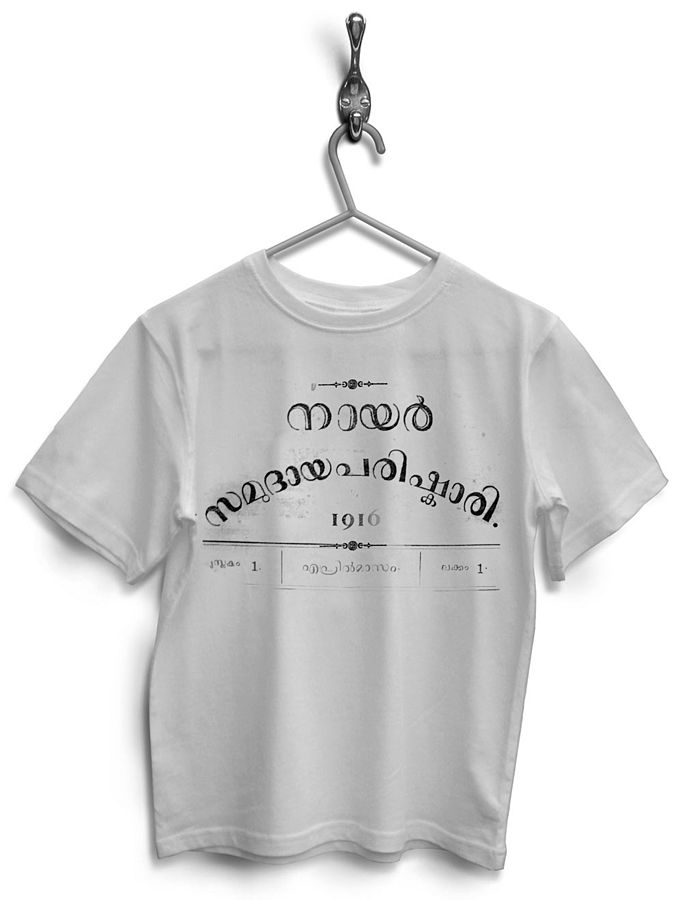
\includegraphics[width=0.6\textwidth,height=10cm]{Kulasthree_Chapter_four_pic08.jpg}
\end{center}
%\caption*{പുലയർ - കെ പി പത്മനാഭ മേനോൻ - വാള്യം 3, (1929), 1984}
\end{figure}

\paragraph{}ബംഗാളിലും മഹാരാഷ്ട്രയിലും വളർന്നു പന്തലിച്ച സാമൂഹ്യപരിഷ്ക്കരണപ്രസ്ഥാനത്തിന്റെ പ്രബലധാരകൾ പലപ്പോഴും ബ്രാഹ്മണമൂല്യങ്ങളെത്തന്നെ ആധുനികരീതിയിൽ പുനഃസൃഷ്ടിക്കാൻ പണിപ്പെടുകയാണുണ്ടായത്. ബ്രാഹ്മണമൂല്യങ്ങളെ തള്ളിക്കളയുന്നതിനു പകരം അവയിലെ നഗ്നമായ അധികാരപ്രയോഗങ്ങളെയും ക്രൂരമായ അംശങ്ങളെയും മാത്രം ഒഴിവാക്കി പുനരുപയോഗിക്കാനാണ് അവ പരിശ്രമിച്ചത്. കൂടാതെ ഈ 'ലഘൂകരിക്കപ്പെട്ട' ബ്രാഹ്മണമൂല്യങ്ങൾ 'പാവന-പുരാതന' 'ഇന്ത്യൻസംസ്ക്കാര'ത്തിന്റെ അവിഭാജ്യഘടകമാണെന്നും ഈ പ്രസ്ഥാനങ്ങളിലെ പ്രബലവിഭാഗങ്ങൾ വാദിച്ചുറപ്പിച്ചു. സ്ത്രീകളുടെ ശരീരങ്ങളുടെമേൽ സൂക്ഷ്മമായ നിയന്ത്രണം ഏർപ്പെടുത്തുകവഴി സമുദായങ്ങളുടെ 'പരിശുദ്ധി' ഉറപ്പുവരുത്താനുള്ള ഉത്സാഹം ഒട്ടുമിക്ക സമുദായപരിഷ്ക്കരണപ്രസ്ഥാനങ്ങളിലും പ്രകടമായിരുന്നു. സ്ത്രീകളുടെ മനഃപരിഷ്ക്കരണത്തിലൂടെവേണം ഇതു സാധിക്കാനെന്ന കാര്യത്തിലും ഇവ തമ്മിൽ വലിയ അഭിപ്രായഭിന്നതയുണ്ടായില്ല; ആധുനികപരിഷ്ക്കാരം സിദ്ധിച്ച പുരുഷന് ഈ പ്രക്രിയയിൽ മേൽക്കൈ നൽകണമെന്ന തീരുമാനത്തെസ്സംബന്ധിച്ചും നല്ല അഭിപ്രായൈക്യം നിലവിലുണ്ടായിരുന്നു!

\paragraph{}സ്വാഭാവികമായും, 'സമുദായപരിഷ്ക്കർത്താവ്' എന്ന അധികാരസ്ഥാനത്തിലേറിയ മലയാളി പുരുഷൻ സ്ത്രീകളെ ആധുനികജീവിതം കെട്ടിപ്പടുക്കുക എന്ന ബൃഹദ്പദ്ധതിയിൽ തന്നോടു തുല്യനിലയുള്ള കൂട്ടാളികളായല്ല കണ്ടത്. മറിച്ച്, പരമ്പരാഗതജീവിതത്തിൽ ആണ്ടുമുങ്ങിക്കിടക്കുന്ന നിസ്സഹായകളാണ് പരമ്പരാഗതസമൂഹത്തിലെ സ്ത്രീകളെന്ന് അയാൾ വിധിച്ചു. ചുരുക്കിപ്പറഞ്ഞാൽ, 'ഗതിയില്ലാത്ത' കുറേ പാവങ്ങളെ രക്ഷപ്പെടുത്താൻ തയ്യാറാകുന്ന ത്യാഗസന്നദ്ധരായിട്ടാണ് സമുദായപരിഷ്ക്കർത്താക്കൾ സ്വയം തിരിച്ചറിഞ്ഞത്. പരിഷ്ക്കരണവസ്തുവായ സ്ത്രീയുടെ നില നിഷ്ക്രിയവും പരിഷ്ക്കർത്താവായ പുരുഷന്റേത് സക്രിയവുമായി സങ്കൽപ്പിക്കപ്പെട്ടു. സ്ത്രീ പുരുഷനു കീഴ്വഴങ്ങി നിൽക്കേണ്ടവൾതന്നെയെന്ന പഴയ പല്ലവിയെ മറ്റൊരുവിധത്തിൽ - കൂടുതൽ സൂക്ഷ്മതയോടെ - പാടുകയായിരുന്നു, സമുദായപരിഷ്ക്കരണപ്രസ്ഥാനങ്ങൾ.
\paragraph{}എന്നാൽ പരമ്പരാഗതകുടുംബങ്ങളിലെ പിതാവ്, അല്ലെങ്കിൽ കാരണവർ, കുടുംബാംഗങ്ങളുടെമേൽ ചെലുത്തിയിരുന്ന അധികാരത്തിൽനിന്ന് തുലോം വ്യത്യസ്തമായ അധികാരമായിരുന്നു പരിഷ്ക്കർത്താവായ പുരുഷന്റേത്. സ്ത്രീയെ ഭയപ്പെടുത്തി അനുസരിപ്പിക്കുന്ന പഴയ രീതിയെ ഉപേക്ഷിച്ചുകൊണ്ടായിരുന്നു ഈ പുതിയ പിതൃമേധാവിയുടെ രംഗപ്രവേശം. സ്ത്രീകളെ അവരുടെ 'യഥാർത്ഥസത്ത' - അതായത്, മേൽവിവരിച്ച 'സ്ത്രീഗുണങ്ങൾ' - വീണ്ടെടുക്കാൻ സഹായിക്കുകയെന്ന ഭാരിച്ച ഉത്തരവാദിത്വം നിർവ്വഹിക്കുവാൻവേണ്ടി ത്യാഗമനുഭവിക്കാൻ തയ്യാറായ പുരുഷന്മാരാണ് പുതിയ പിതൃമേധാവിത്വത്തിന്റെ വക്താക്കളും പ്രയോക്താക്കളുമായിത്തീർന്നത്. ബലപ്രയോഗത്തിലൂടെയല്ല, മറിച്ച്, മനഃപരിഷ്ക്കരണത്തിലൂടെവേണം സ്ത്രീകളെ ഉത്തമ വീട്ടമ്മമാരാക്കിമാറ്റാനെന്ന നിർദ്ദേശം പുതിയ പിതൃമേധാവികൾ പരക്കെ അംഗീകരിച്ചിരുന്നു. പരമ്പരാഗത കുടുംബത്തിൽനിന്നും ആധുനിക കുടുംബത്തിലേക്ക് സ്ത്രീയെ കൈപിടിച്ചുയർത്തുന്ന ക്ലേശകരമായ ഉത്തരവാദിത്വം ഏൽക്കുന്നതുകൊണ്ട് പുരുഷനു ചില ഗുണങ്ങളുണ്ടായിരുന്നു: തന്റെ പരിഷ്ക്കരണവസ്തുക്കളായ സ്ത്രീകളുടെമേൽ ഒടുങ്ങാത്ത ധാർമ്മികാധികാരം അയാൾക്കു കൈവന്നു. നവപിതൃമേധാവിത്വത്തിന്റെ വക്താക്കളായിരുന്ന പല പുരുഷപരിഷ്ക്കർത്താക്കന്മാർക്കും 'സ്ത്രീവിമോചക'രെന്ന ബിരുദം കൈവന്നത് അങ്ങനെയാണ്.

\paragraph{}പരമ്പരാഗതപിതൃമേധാവിത്വത്തിന്റെ കരാളഹസ്തങ്ങളിലകപ്പെട്ടുപോയ സ്ത്രീയെ രക്ഷപ്പെടുത്തി പരിഷ്ക്കരിച്ച് 'ആധുനികസ്ത്രീ'യാക്കാൻ പണിപ്പെട്ട പുരുഷനായ പരിഷ്ക്കർത്താവിന്റെ ഉത്തരവാദിത്വത്തെ ആസ്പദമാക്കി രചിക്കപ്പെട്ട അതിപ്രശസ്തമായ നാടകമായിരുന്നു വി.ടി. ഭട്ടതിരിപ്പാടിന്റെ അടുക്കളയിൽനിന്ന് അരങ്ങത്തേക്ക് (1930). നമ്പൂതിരിസമുദായപരിഷ്ക്കരണപ്രസ്ഥാനത്തിലെ സുപ്രധാനസംഭവങ്ങളിലൊന്നായിരുന്നു ഈ നാടകത്തിന്റെ അവതരണം. പരമ്പരാഗതസമുദായത്തിന്റെ പോഴത്തങ്ങളെ കണക്കിനു പരിഹസിച്ച ഈ നാടകം സമുദായത്തിനുള്ളിലും പുറത്തും വലിയ ഒച്ചപ്പാടുണ്ടാക്കി. പരമ്പരാഗതപിതൃമേധാവിത്വത്തിന്റെ പിടിയിൽ ഞെരിഞ്ഞമർന്നു നശിച്ചുപോകുമായിരുന്ന ഒരു യുവതിയെ പരിഷ്കൃതനായ ഒരു നമ്പൂതിരിയുവാവ് രക്ഷപ്പെടുത്തി ഒരു പുതിയ ജീവിതത്തിലെത്തിക്കുന്ന കഥയിൽ പരിഷ്ക്കർത്താവിനാണ് സജീവമായ പങ്ക്. പരിഷ്കൃതനായ പുരുഷന്റെ സഹായമില്ലെങ്കിൽ സ്ത്രീ മരിക്കുകയോ ഭ്രാന്തിയാവുകയോ ചെയ്യുമെന്ന് സൂചിപ്പിക്കുന്ന പല 'നമ്പൂതിരി സമുദായപരിഷ്ക്കരണ'കഥകളും ഇക്കാലത്തുണ്ടായിട്ടുണ്ട്. സ്ത്രീവിമോചകരായ പുരുഷപരിഷ്ക്കർത്താക്കളുടെ കടമയെ ചുറ്റിപ്പറ്റിയുള്ള പ്രമേയങ്ങൾ മറ്റു സമുദായങ്ങളുടെ പശ്ചാത്തലത്തിലും അവതരിപ്പിക്കപ്പെട്ടിട്ടുണ്ട് - പലപ്പോഴും വ്യതിയാനങ്ങളോടെ. ഉദാഹരണത്തിന് വി.ടി.യുടെ പ്രശസ്ത കൃതിയുടെ പേര് അടുക്കളയിൽനിന്ന് അരങ്ങത്തേക്ക് എന്നാണെങ്കിലും അതിലെ നായികയുടെ യാത്ര അടുക്കളയിൽനിന്ന് വീട്ടിന്റെ പൂമുഖത്തേക്കാണ്. എന്നാൽ മലബാറിൽ ഏറെ പ്രശസ്തിനേടിയ ഇതു ഭൂമിയാണ് എന്ന നാടകത്തിലെ നായിക അടുക്കളയിൽനിന്ന് നാടകത്തിന്റെ അരങ്ങത്തേക്കുതന്നെയാണ് സഞ്ചരിക്കുന്നത്. രണ്ടിലും രക്ഷകസ്ഥാനത്ത് പരിഷ്ക്കർത്താവായ പുരുഷൻതന്നെ.

\paragraph{}ഒറ്റനോട്ടത്തിൽ ഇത് അനിവാര്യമായിരുന്ന ഒരു അധികാരബന്ധമായിരുന്നുവെന്ന് തോന്നിയേക്കാം. പഠിപ്പും ലോകപരിചയവും കുറഞ്ഞവർക്ക് പൊതുരംഗത്തേക്കു കടക്കാൻ ഇതുരണ്ടും സമ്പാദിച്ചുകഴിഞ്ഞവരുടെ സഹായം വേണ്ടിവരുമെന്ന് പ്രതീക്ഷിക്കേണ്ടതല്ലേ? ഒരളവുവരെ ഇതു ശരിയാണെന്ന് സമ്മതിക്കാം. എന്നാൽ ആ സഹായഹസ്തം അധികാരബന്ധമായിത്തീരാനിടയുണ്ടെന്ന് അക്കാലത്തെ അന്തർജനങ്ങൾതന്നെ മുൻകൂട്ടിക്കണ്ടിരുന്നു. നമ്പൂതിരിസമുദായപ്രസ്ഥാനത്തിന്റെ പ്രസിദ്ധീകരണമായ യോഗക്ഷേമത്തിലും മറ്റും സ്ത്രീകളെക്കുറിച്ചെഴുഴുതിയ പല അന്തർജനങ്ങളും ഇതു പരോക്ഷമായി സൂചിപ്പിച്ചു. സ്ത്രീകളെ പരിഷ്ക്കരിക്കൽ പുരുഷന്മാർ സ്ത്രീകളോടു കാണിക്കുന്ന ഔദാര്യമല്ലെന്നും സ്ത്രീകൾ അഭ്യസ്തവിദ്യകളായിത്തീർന്നില്ലെങ്കിൽ അതുകൊണ്ടുള്ള ദോഷം അവരെമാത്രമല്ല പുരുഷന്മാരെയും ബാധിക്കുമെന്നും ഇവർ പലപ്പോഴും ഓർമ്മിപ്പിച്ചു.

\captionof{mybox}{ഇത് ഭൂമിയാണ്}\label{ch4box4} % place the caption
\begin{tcolorbox}[%
 breakable, % make the box breakable
  arc=0mm, 
  left=1pt, right = 1pt, 
  boxrule=0mm,
  colback = {blue!10}, % since shadow-gray was not defined
] 
\noindent

മലയാളത്തിലെ ഏറ്റവും പ്രശസ്തമായ മുസ്ലിം സാമൂഹ്യനാടകമാണ് കെ.ടി. മുഹമ്മദിന്റെ ഇതു ഭൂമിയാണ്. (1953) മുസ്ലിംസ്ത്രീകളെ നേരിട്ട് അഭിസംബോധനചെയ്യുകയും അവരുടെ പ്രശ്നങ്ങളെ വെളിച്ചത്തു കൊണ്ടുവരികയും ചെയ്ത നാടകമാണിത്. വൈക്കം മുഹമ്മദ് ബഷീറിന്റെ ബാല്യകാലസഖി (1944), ന്റുപ്പുപ്പക്കാക്കൊരാനേണ്ടാർന്നു! (1951) എന്നീ കൃതികൾ മുസ്ലിംസ്ത്രീകളുടെ ദൈനംദിനജീവിതത്തെ സാമൂഹ്യപരിഷ്ക്കരണ കാഴ്ചപ്പാടിൽനിന്ന് വിലയിരുത്തിയവയായിരുന്നു; ആ പരമ്പരയിലാണ് ഇതു ഭൂമിയാണ് എന്ന നാടകത്തിന്റെയും സ്ഥാനം. സ്ത്രീവിദ്യാഭ്യാസമാണ് ഈ നാടകത്തിലേയും മുഖ്യപ്രമേയം. ഇന്നും മുസ്ലിംസ്ത്രീകൾ നേരിടുന്ന പല പ്രശ്നങ്ങളും ഈ നാടകം ചർച്ചചെയ്യുന്നുണ്ട് - ബഹുഭാര്യാത്വം, പുരുഷന് ഭാര്യയെ ഏകപക്ഷീയമായി മൊഴിചൊല്ലാനുള്ള സൗകര്യം, സ്ത്രീകളുടെ സ്വത്തുടമസ്ഥതയുടെ പ്രശ്നം - എല്ലാം. എന്നാൽ പൊതുവെ മുസ്ലിംസമുദായപരിഷ്ക്കരണവും ഇവിടെ വിവരിച്ച പുതിയ ലിംഗാധികാരബന്ധത്തെ ഊട്ടിയുറപ്പിക്കുകയായിരുന്നുവെന്ന് സമീപകാലസ്ത്രീപക്ഷചരിത്രഗവേഷണം വെളിവാക്കുന്നു. മുൻ അദ്ധ്യായത്തിൽ പരാമർശിച്ച പുത്തൂർ ആമിനയുടെ പാട്ടിലെ സ്ത്രീസ്വാതന്ത്ര്യാദർശമല്ല പുരുഷന്മാരായ മുസ്ലിംസമുദായപരിഷ്ക്കർത്താക്കന്മാരുടേത് എന്ന് ഷംഷാദ് ഹുസൈൻ ചൂണ്ടിക്കാണിക്കുന്നു. മുസ്ലിം ഐക്യസംഘം എന്ന സുപ്രസിദ്ധ പരിഷ്ക്കരണസംഘടനയുടെ ആദർശങ്ങൾ സമുദായനവീകരണത്തെ ഉന്നംവച്ച് സ്ത്രീകളെ എങ്ങനെ പരിഷ്ക്കരിക്കണമെന്ന് നിർദ്ദേശിക്കുന്നവയായിരുന്നു. 
\begin{quotation}
\noindent 'കാതുകുത്തുപോലുള്ള അനിസ്ലാമിക ദുരാചാരങ്ങളെ എതിർക്കുക... പൗരോഹിത്യം വിലക്കിയ സ്ത്രീവിദ്യാഭ്യാസം നടപ്പിലാക്കുക എന്നിങ്ങനെ. സമുദായത്തിനുവേണ്ടി സ്ത്രീകൾ എങ്ങനെയെല്ലാം പരിഷ്ക്കരിക്കപ്പെടണം എന്നതാണ് ഇവയിലെ മുഖ്യ അജണ്ട. അല്ലാതെ സ്ത്രീയുടെ വീക്ഷണകോണിൽനിന്നുകൊണ്ടുള്ള സ്ത്രീസമുദായപരിഷ്ക്കരണങ്ങളല്ല.' 
\flushright{(ഷംഷാദ് ഹുസൈൻ, ന്യൂനപക്ഷത്തിനും ലിംഗപദവിക്കുമിടയിൽ, തിരുവനന്തപുരം, 2009, പുറം. 24)}
\end{quotation}
\end{tcolorbox}


\begin{figure}[h]
\begin{center}
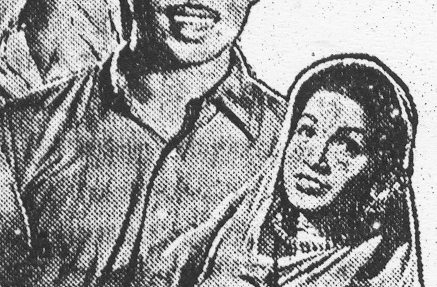
\includegraphics[width=0.9\textwidth,height=10cm]{Kulasthree_Chapter_four_pic09.jpg}
\end{center}
%\caption*{പുലയർ - കെ പി പത്മനാഭ മേനോൻ - വാള്യം 3, (1929), 1984}
\end{figure}

\paragraph{}ഈ സഹായഹസ്തം വലിയൊരു അധികാരബന്ധംതന്നെയായിരുന്നുവെന്ന് നമ്പൂതിരിപരിഷ്ക്കർത്താക്കളിൽ അഗ്രഗണ്യനായിരുന്ന വി.ടി ഭട്ടതിരിപ്പാടിന്റെ ചില രചനകളിൽനിന്നു വ്യക്തമാകുന്നുണ്ട്. അന്തർജനങ്ങളുടെ നരകജീവിതത്തെക്കുറിച്ച് ഏറ്റവുമധികം എഴുതിയിട്ടുള്ള ഒരാളാണ് അദ്ദേഹം. എഴുത്തും വായനയും പഠിച്ച് യുക്തിചിന്തയിലേക്കുയർന്ന് ഇല്ലങ്ങളിലെ ഇടുങ്ങിയ അന്തരീക്ഷത്തിൽനിന്ന് സ്വന്തം മനസ്സിനെ വിമോചിപ്പിക്കാൻ അന്തർജനങ്ങൾ സ്വയം തയ്യാറാവണമെന്ന് ശക്തമായി വാദിച്ചയാൾ. (കാണുക \ref{umadevi}) എന്നാൽ പരിഷ്ക്കർത്താവായ പുരുഷൻ നീട്ടിയ സഹായഹസ്തത്തെ ഏതെങ്കിലും അന്തർജനം സ്വീകരിക്കാതിരുന്നാൽ, അവൾ ഇല്ലത്തിനുപുറത്തേക്ക് സ്വന്തം വഴി തേടിയാൽ, ക്ഷമിക്കാൻ പറ്റാത്ത അപരാധമായി അതെണ്ണപ്പെടുമെന്ന് വി.ടിയുടെ കർമ്മവിപാകം എന്ന ആത്മകഥാപരമായ ലേഖനസമാഹാരത്തിലുൾപ്പെടുത്തിയിട്ടുള്ള ഒരു ലേഖനം വെളിവാക്കുന്നുണ്ട്. 

\paragraph{}
\label{uma-vt}
	ഉമാദേവി നരിപ്പറ്റ എന്ന സ്ത്രീയെക്കുറിച്ച് വി.ടിയുടെ ഓർമ്മക്കുറിപ്പാണത് - വലിയൊരു കുറ്റപത്രംതന്നെ വി.ടി. അവർക്കെതിരെ സമർപ്പിക്കുന്നുണ്ട്. അനുസരണയും ധർമ്മബോധവുമില്ലാത്ത, അമിതലാളനകൊണ്ട് വെറും വഷളായ, ഒരു സ്ത്രീയാണവർ, വി.ടിയുടെ വീക്ഷണത്തിൽ. പക്ഷേ, വി.ടിയടക്കമുള്ള സമുദായ വിപ്ലവകാരികൾ എതിർത്തുതോൽപ്പിച്ച യാഥാസ്ഥിതിക കുടുംബസാഹചര്യത്തിൽനിന്നാണ് അവർ ഇറങ്ങിപ്പോയതെന്ന് സുവ്യക്തമാണ് - ഭർത്തൃപിതാവ് അവരുടെ ഭർത്താവിനെക്കൊണ്ട് രണ്ടാമത് വേളികഴിപ്പിച്ചത്രെ. സപത്നിയായിവന്ന സ്ത്രീക്ക് ആദ്യഭാര്യയായ ഉമയിൽനിന്ന് ഭർത്താവിന്റെ പങ്ക് നേടിയെടുക്കാനായില്ലത്രേ. കൗതുകവസ്തുക്കൾ മോഷ്ടിക്കുന്ന സ്വഭാവം ഉമയ്ക്കുണ്ടായിരുന്നെന്നും അതിനു പ്രായശ്ചിത്തം ചെയ്യാൻ ഭർത്തൃപിതാവ് നിർബന്ധിച്ചപ്പോൾ അനുസരിക്കാതെ കുട്ടികളെയെടുത്തുകൊണ്ട് അവർ വീടുവിട്ടിറങ്ങിയെന്നും വി.ടി പറയുന്നു. ഇവിടെ വി.ടി ക്ക് യാതൊരു സംശയവുമില്ല - യാഥാസ്ഥിതികനായ നമ്പൂതിരികാരണവരുടെ ആരോപണത്തെക്കുറിച്ച്, കളവെന്ന ദുഃസ്വഭാവത്തെ പരിഹരിക്കാൻ അയാൾ നിർദ്ദേശിച്ച മാർഗ്ഗത്തെക്കുറിച്ച്. ഒറ്റയ്ക്ക് ഇറങ്ങിപ്പോയി എന്നതുതന്നെയാണ് ഉമ തെറ്റുചെയ്തുവെന്നതിന്റെ തെളിവ്. ഇല്ലത്തുനിന്നിറങ്ങിയശേഷം ഉമയ്ക്ക് നിരവധി കാമുകന്മാരുണ്ടായെന്ന്, അന്യജാതിക്കാരായ പുരുഷന്മാരുടെകൂടെ അവർ പുതിയജീവിതം ആരംഭിക്കാൻ ശ്രമിച്ചുവെന്ന് പറയുന്ന വി.ടിയുടെ ദൃഷ്ടിയിൽ ക്ഷമയർഹിക്കാത്ത കുറ്റമാണ് ആ ഇറങ്ങിപ്പോക്ക്. പരിഷ്ക്കർത്താവായ പുരുഷന്റെ മേൽനോട്ടത്തിലല്ല അവർ ഈ നീക്കങ്ങൾ നടത്തിയതെന്നതാണ് യഥാർത്ഥപ്രശ്നം - വി.ടിയുടെ സഹോദരിയെ അദ്ദേഹത്തിന്റെ മേൽനോട്ടത്തിലും താൽപ്പര്യത്തിലും ഒരു നായർ വിവാഹം കഴിച്ചതിനെക്കുറിച്ചും അദ്ദേഹമെഴുതിയിട്ടുണ്ട്. അഭിജാതമായ ഇല്ലത്തുനിന്ന് ദരിദ്രമായ ഒരു മാപ്പിളഗൃഹത്തിലേക്ക് ഇറങ്ങിപ്പോയ അന്തർജനത്തെ എത്ര ശകാരിച്ചിട്ടും വി.ടി.ക്കു മതിവരുന്നില്ല. അതിന്റെ കുറ്റമത്രയും 'സ്ത്രീസ്വാതന്ത്ര്യത്തിന്റെ തലയിൽ കെട്ടിവയ്ക്കാനും അദ്ദേഹം മറക്കുന്നില്ല - സ്ത്രീകളെ വിമോചിപ്പിക്കാൻ നടന്നവർ 'സ്ത്രീസ്വാതന്ത്ര്യ'ത്തെ ഭയപ്പെടുന്നതിലെ വിരോധാഭാസം ചില്ലറയല്ല! സ്വസമുദായത്തിനുള്ളിൽ, പുരുഷന്മാരായ പരിഷ്ക്കർത്താക്കൾ വരച്ചവരയ്ക്കകത്ത്, അവർ തീർത്ത നിയമങ്ങളനുസരിച്ചുമാത്രമേ 'സ്ത്രീസ്വാതന്ത്ര്യം' പാടുള്ളൂ എന്നർത്ഥം.


\begin{quotation}
\noindent
സ്ത്രീസ്വാതന്ത്യ്രം പൂവിടുന്ന വസന്തം പിറന്നതിന്റെ നറുമണം ഉമാ അന്തർജനത്തെ ലഹരിപിടിപ്പിച്ചു. സദാചാരത്തിന്റെ വഴിയിൽ അവൾക്കു കാലിടറാൻ തുടങ്ങി. കാമുകജനത്തിനു ബഹുരസം. ചിലർ കൈമുട്ടി പ്രോത്സാഹിപ്പിച്ചു. ഇന്നവിടെ, നാളെ മറ്റൊരിടത്ത് - അങ്ങനെ അവർ ഒളിച്ചുകളിച്ചു. ഈ അപഥസഞ്ചാരത്തിൽനിന്നു വ്യതിചലിപ്പിക്കുവാൻ സാദ്ധ്യമല്ലെന്നായപ്പോൾ അവളുടെ ഭർത്തൃഗൃഹക്കാരും പിതൃഗൃഹക്കാരും ബാദ്ധ്യത ഒഴിവാക്കാൻ മുന്നോട്ടുവന്നു. രജിസ്ട്രാഫീസിൽ ജനം കൂടി. ഭർത്തൃഗൃഹത്തിന്റെ പ്രതിനിധിയായി മദ്ധ്യസ്ഥന്മാരുടെ മുമ്പിൽ ഹാജരായ ഒരു ഇരിക്കണമ്മയുടെ (നമ്പൂതിരി ഇല്ലത്തെ നായർ പരിചാരിക) വശം ഉമാ അന്തർജനം മുലകുടിച്ചു തോളിൽ ചാഞ്ഞുറങ്ങുന്ന ആൺകുഞ്ഞിനെ കൈമാറിയപ്പോൾ നോക്കിനിന്നവരുടെ കണ്ണുകൾ നനഞ്ഞുപോയി.
\flushright{(വി.ടി.യുടെ സമ്പൂർണ്ണ കൃതികൾ, കോട്ടയം, 2006, പുറം 323-24)}
\end{quotation}

\paragraph{}ഉമയുടെ മകളെ ഭർത്തൃവീട്ടുകാർ എന്തുകൊണ്ട് ആവശ്യപ്പെട്ടില്ലെന്ന ചോദ്യം വി.ടി. ചോദിക്കുന്നില്ല; ഒന്നിലധികം വേളികഴിച്ച ഉമയുടെ ഭർത്താവ് കുറ്റക്കാരനല്ലാത്തപ്പോൾ ഒരു ഭർത്താവിനെ വേണ്ടെന്നുവച്ചശേഷംമാത്രം മറ്റൊരാളെ വരിച്ച ഉമ കുറ്റക്കാരിയാവുന്നതെങ്ങനെ എന്നും ചോദിക്കുന്നില്ല. 'തറവാട്ടിൽ പിറന്നവൾ' 'ചന്തപ്പെണ്ണാ'യിത്തീർന്നതിൽ അടക്കാനാവാത്ത രോഷം പ്രകടിപ്പിക്കുന്നതിനിടയിൽ അതിനൊന്നും സമയമില്ല!

\paragraph{}ഉമാദേവി അന്തർജനങ്ങൾക്കു മാതൃകയല്ലെന്ന് പലതരത്തിൽ പറയാൻ നമ്പൂതിരി പരിഷ്ക്കർത്താക്കൾ ശ്രദ്ധിച്ചിരുന്നു (അവർ ആർക്കെങ്കിലും മാതൃകയാകാൻ ശ്രമിച്ചിരുന്നോ എന്നത് വേറെകാര്യം - അവരുടെ തീരുമാനങ്ങൾ ഏതുസാഹചര്യത്തിൽ കൈക്കൊണ്ടവയാണെന്നും നമുക്കറിയില്ല!) എം.പി. ഭട്ടതിരിപ്പാടിന്റെ ഋതുമതി (1940) എന്ന പ്രശസ്ത സമുദായപരിഷ്ക്കരണനാടകത്തിൽ ഇവർ 'പ്രത്യക്ഷപ്പെടുന്നുണ്ട്.' ഇതിലെ നായിക ദേവകി എന്ന പെൺകുട്ടിയാണ്. അവൾ തന്റെ ഇല്ലത്തെ യാഥാസ്ഥിതിക അന്തരീക്ഷത്തിനെതിരെ ഉറച്ചുനിൽക്കാൻ തീരുമാനിക്കുന്നു. പക്ഷേ, ഉമാ അന്തർ ജനത്തെപ്പോലെയല്ല താനെന്നും ഇല്ലത്തുനിന്നു പുറത്തുപോയാൽ അത് സഹോദരസ്ഥാനീയനായ ബന്ധുവിന്റെയൊപ്പമായിരിക്കുമെന്നും പ്രഖ്യാപിക്കുന്നു!

\paragraph{}പുരുഷപരിഷ്ക്കർത്താക്കളുടെ ഈ മനോഭാവത്തെ അന്നുതന്നെ സാഹിത്യരംഗത്ത് പ്രശസ്തിയാർജ്ജിച്ചുകഴിഞ്ഞിരുന്ന ലളിതാംബികാ അന്തർജനം തന്റെ 'പ്രസാദം' (1939) എന്ന കഥയിൽ രൂക്ഷമായി വിമർശിക്കുന്നുണ്ട്. നമ്പൂതിരിസമുദായപരിഷ്ക്കരണപ്രസ്ഥാനത്തെ അനുകൂലിച്ച് നിരവധി കഥകൾ രചിച്ച അന്തർജനം, ഈ കഥയിലൂടെ അതിനെ കഠിനമായി വിമർശിച്ചു - പരമ്പരാഗതജീവിതത്തിൽനിന്ന് സ്ത്രീകളെ രക്ഷിക്കാൻ പുറപ്പെട്ടവർതന്നെ പുതിയ പിതൃമേധാവിത്വത്തിന്റെ വാഹകരായിത്തീർന്ന പ്രക്രിയയെ അവർ ഈ കഥയിലൂടെ വരച്ചുകാട്ടുന്നു. ഒരിടയ്ക്ക് സമുദായവിപ്ലവകാരിണിയായി പേരെടുത്ത ഒരു നമ്പൂതിരിസ്ത്രീ പെട്ടെന്ന് സ്വകാര്യജീവിതത്തിലേക്കും പ്രാർത്ഥനയിലേക്കും പിൻവാങ്ങുന്നതിന്റെ കഥയാണിത്. അവരുടെ ഈ പ്രവൃത്തി പുരുഷന്മാരായ പരിഷ്ക്കർത്താക്കളെ ചൊടിപ്പിക്കുന്നു. തങ്ങൾ പ്രസംഗം പഠിപ്പിച്ചു പീഠത്തിലേറ്റിയവൾ ഇപ്പോൾ യാതൊരു നന്ദിയുംകൂടാതെ എല്ലാം ഉപേക്ഷിച്ചുപോയതിൽ അവർ രോഷം പ്രകടിപ്പിക്കുന്നു. പുരുഷപരിഷ്ക്കർത്താവിന് പരിഷ്ക്കരണവസ്തുവായ സ്ത്രീയുടെമേലുള്ള ധാർമ്മികാധികാരമാണ് ഇവിടെ ചോദ്യവിധേയമാകുന്നത്:

\begin{quotation}
\noindent കാര്യപരിപാടിയിലെ കാര്യമായ ഒരിനത്തിൽ പങ്കുകൊള്ളാനവർക്കെന്തുകൊണ്ടോ കഴിഞ്ഞില്ല. അതൊരു സൂത്രമായി ചിലർ വ്യാഖ്യാനിച്ചു... ക്ഷുഭിതനായ ഒരു യുവാവ് പറഞ്ഞു: "ഈ മരപ്പാവകളെ ഉദ്ധരിക്കുവാൻവേണ്ടിയാണല്ലോ ഞങ്ങളീ പാടൊക്കെപ്പെട്ടത്. ഓരോരുത്തരെ പഠിപ്പിച്ചു... പ്രസംഗിച്ചു പേരുംകൊടുത്തപ്പോൾ കണ്ടില്ലേ ആ നന്ദി..."

\noindent
ഈ വാദം വാസ്തവമല്ലേ? നമ്മുടെ പുരുഷന്മാർക്ക് നീക്കംചെയ്യേണ്ടതായി എന്തൊരവശതയാണുള്ളത്. സമുദായപ്രവർത്തനങ്ങളുടെ ആവശ്യംതന്നെയെന്ത്? ഇവരുടെ കനിവില്ലെങ്കിൽ വല്ലതും നടക്കുമോ?... എന്നാലും ഈ നന്ദിയെപ്പറ്റിയുള്ള സൂചന എന്നെ ക്ഷുബ്ദ്ധയാക്കി. നന്ദിപോലും... നാണംകെട്ട ഒരു പദം... ഭാരമേറിയ കടപ്പാട്... അടിമത്തത്തിലും കഷ്ടതരം...

\flushright{('പ്രസാദം', ലളിതാംബിക അന്തർജനത്തിന്റെ കഥകൾ സമ്പൂർണ്ണം, കോട്ടയം, 2009, പുറം 179)}
\end{quotation}


\paragraph{}പുരുഷനായ പരിഷ്ക്കർത്താവിന്റെ നിലയെക്കുറിച്ച് അക്കാലത്ത് സ്ത്രീകൾക്കിടയിൽത്തന്നെ ഭിന്നാഭിപ്രായങ്ങൾ നിലനിന്നിരുന്നുവെന്നതിൽ സംശയമില്ല. പരിഷ്ക്കർത്താവിന്റെ അധികാരം സ്ത്രീയെ പൂർണ്ണസ്ത്രീത്വത്തിലേക്കല്ല, പൂർണ്ണവ്യക്തിത്വത്തിലേക്കുയർത്താൻ ഉതകിയാൽ, അത് ഗുണകരംതന്നെ എന്നായിരുന്നു കെ. സരസ്വതിയമ്മയുടെ അഭിപ്രായം. (കാണുക \ref{saraswathy}) അങ്ങനെയെങ്കിൽ പുരുഷന്റെ അധികാരം അൽപ്പായുസ്സായിരിക്കുമെന്നും, സ്ത്രീപുരുഷതുല്യത പുരുഷന്റെ ജീവിതത്തിന്റെ നിലവാരത്തെയും ഉയർത്തുമെന്നും അവർ വാദിച്ചു. താൻ ഒരു ഭർത്താവായിരുന്നെങ്കിൽ, തന്റെ ഭാര്യയെ എങ്ങനെ പരിഷ്ക്കരിക്കുമെന്നതിനെക്കുറിച്ച് അവരെഴുതിയ ലേഖനത്തിൽനിന്ന്:
\begin{quotation}
\noindent വെറും പുരുഷനെന്ന നിലയിൽ സ്ത്രീസ്വാതന്ത്ര്യത്തെയും സമത്വത്തെയും സ്വാഗതം ചെയ്യുന്നതൊരു സുഖമാണ്... പക്ഷേ, ഭർത്താവിന്റെ നിലയിലായാലോ?

\noindent
....പരമ്പരാഗതമായി പകർന്നുകിട്ടിയിട്ടുള്ള ആചാരക്രമങ്ങൾ, അന്ധവിശ്വാസങ്ങൾ, മഹദ്വാക്യങ്ങൾ അത്രവേഗം ഇടിച്ചു നിരത്താനാവുമോ? കെട്ടിയുറപ്പിച്ചതു സ്വാർത്ഥമതികളായ നമ്മൾ; ഇടിച്ചുനിരത്തേണ്ടത് അസ്വതന്ത്രകളായ അബലകൾ. മഹാമനസ്കരായ നമ്മിൽ ചിലർ ഇടയ്ക്കൊക്കെ അൽപ്പാൽപ്പം സഹായിക്കുന്നു എന്നുമാത്രം...

\noindent
...കണ്ണീരൊഴുക്കി കാര്യംകാണാനും അസൂയകൊണ്ട് അയൽപെണ്ണുങ്ങളെ ദുഷിക്കാനും മൃദുലവികാരങ്ങളിൽ മുങ്ങിനശിക്കാനും മറ്റുമൊക്കെയാണു സ്ത്രീകൾക്കു വാസന എന്നു നാം പറയുമ്പോൾ, അതിനുള്ള പരിതഃസ്ഥിതി നാമാണു സൃഷ്ടിച്ചുകൊടുത്തത് എന്നകാര്യം നാം ഓർമ്മിക്കാറുണ്ടോ? കർമ്മധീരതയുണ്ടാവാനും ബുദ്ധിശക്തി വികസിപ്പിക്കാനും നാം അവരെ അനുവദിച്ചില്ലെന്നു മാത്രമല്ല, അതൊരപകർഷമായി ഗണിക്കുകപോലും ചെയ്തില്ലേ? സ്ത്രീയിൽ വൈകാരികഭാവം പരിധിയില്ലാതെ വളർത്തി അവളുടെ ബുദ്ധിയെക്കൂടെ ഹൃദയമാക്കി മാറ്റാൻ നിരന്തരം ശ്രമിച്ച നാം പാവയെന്നും കളിക്കോപ്പെന്നും അവരെ പുച്ഛിക്കുന്നതിനർത്ഥമുണ്ടോ?
\flushright{(കെ. സരസ്വതിയമ്മയുടെ സമ്പൂർണ്ണകൃതികൾ, കോട്ടയം, 2001, പുറം 986-87)}
\end{quotation}


ഇവിടെ ഭർത്താവ് പരിഷ്ക്കർത്താവിന്റെ നില സ്വീകരിക്കണമെന്നാണ് സരസ്വതിയമ്മ നിർദ്ദേശിക്കുന്നത്. പക്ഷേ, പരിഷ്ക്കരണത്തിന്റെ ലക്ഷ്യം സ്ത്രീത്വമുണ്ടാക്കലല്ല, സ്ത്രീയെ പൂർണ്ണവ്യക്തിത്വത്തിലെത്തിക്കലാണ്.
1930കളോടെ പരിഷ്ക്കരണപ്രസ്ഥാനങ്ങളിൽ പ്രമുഖരായ പല സ്ത്രീകളും ഉയർന്നുവന്നു - ആര്യാപള്ളം, ദേവകി നരിക്കാട്ടിരി, പാർവ്വതി നെന്മിനിമംഗലം മുതലായ നമ്പൂതിരിസ്ത്രീകൾ,(കാണുക \ref{ch7box2} ) തോട്ടയ്ക്കാട്ടു മാധവിയമ്മ, (കാണുക \ref{ch10box3})കോന്നിയൂർ മീനാക്ഷിയമ്മ മുതലായ നായർസ്ത്രീകൾ, ഗൗരീ പവിത്രൻ, മുതുകുളം പാർവ്വതിയമ്മ തുടങ്ങിയ ഈഴവസ്ത്രീകൾ, സി. രുദ്രാണിയെപ്പോലുള്ള അരയസ്ത്രീകൾ - ഇവരെല്ലാം പൊതുരംഗത്ത് സജീവസാന്നിദ്ധ്യമായിത്തീർന്നു. ഇവരുടെ നിലയ്ക്ക്, പക്ഷേ, വല്ലാത്തൊരനിശ്ചിതത്വമുണ്ടായിരുന്നു. ഒരുവശത്ത് സ്ത്രീകളെ 'ഉദ്ധരിക്കാനു'ള്ള ചുമതലയിൽ പങ്കുവഹിച്ച ഇവർക്ക് പലപ്പോഴും മറുവശത്ത് പുരുഷപരിഷ്ക്കർത്താളോട് വിധേയത്വം കാട്ടേണ്ടിവന്നു. ഇങ്ങനെ അധികാരത്തിനും അധികാരമില്ലായ്മയ്ക്കുമിടയിൽ ചാഞ്ചാടിയുള്ള ജീവിതംമടുത്ത് സ്വന്തംവീട്ടിലേക്കു മടങ്ങിയ ഒരു സ്ത്രീയുടെ കഥയാണ് ലളിതാംബിക അന്തർജനം 'പ്രസാദ'ത്തിൽ പറഞ്ഞത്. എന്നാൽ ഈ നിലയെ നിസ്സംശയം തള്ളിക്കളഞ്ഞ സ്ത്രീകളായ പരിഷ്ക്കർത്താക്കൾ ആ തലമുറയിൽ ഉണ്ടായിരുന്നു - അവരെക്കുറിച്ച് നാമധികം ഇന്നു കേൾക്കാറില്ലെങ്കിലും. അന്നു പ്രശസ്തയായിരുന്ന പാർവ്വതി അയ്യപ്പൻ അവരിലൊരാളായിരുന്നു. ഗൃഹകാര്യങ്ങൾ നോക്കുന്നതിൽ കഴിവുനേടുക മാത്രമല്ല സ്ത്രീയുടെ ധർമ്മമെന്ന് അവർ അഭിപ്രായപ്പെട്ടു:


\begin{quotation}
വർഗ്ഗം നിലനിറുത്തിക്കൊണ്ടുപോകുന്നതിനു പ്രകൃതി വ്യക്തികളിൽ ചില വാസനകളും വളർത്തിക്കൊണ്ടുവന്നിട്ടുണ്ട്. ആ വാസനകളുടെ പ്രേരണാഫലമായി ചില സ്ത്രീപുരുഷബന്ധങ്ങളുമുണ്ടായിട്ടുണ്ട്. അവയുടെ നാഗരികമായ ഒരു പരിണാമമാണു ഭാര്യാഭർതൃബന്ധവും പരിഷ്കൃതഗൃഹജീവിതവും. സ്ത്രീക്കും പുരുഷനും ഇതിലും കവിഞ്ഞ പല ധർമ്മങ്ങളും നിറവേറ്റാനുണ്ട്. മനുഷ്യസമുദായത്തിന്റെ പുരോഗതിക്കു സ്ത്രീകളും പുരുഷന്മാരും ഒരുപോലെ വേലചെയ്യണം. അതിന് ഏറ്റവും ആവശ്യമായിട്ടുള്ളതു സ്ത്രീയിലും പുരുഷനിലും അന്തർലീനമായിക്കിടക്കുന്ന ബുദ്ധിപരമായും മറ്റുമുള്ള കഴിവുകളെ ആവിഷ്ക്കരിക്കയാണ്. ആ സംഗതിയിൽ സ്ത്രീപുരുഷഭേദമില്ല... കഴിയുന്നതും ഭർത്താക്കന്മാരുടെ വേലകളിൽ സഹകരിക്കുന്ന ഭാര്യമാരും ഭാര്യമാരുടെ വേലകളിൽ സഹകരിക്കുന്ന ഭർത്താക്കന്മാരും യോജിക്കുന്ന ദാമ്പത്യങ്ങളാണ് ഉത്തമമായിട്ടുള്ളത്.
\flushright{ (പാർവ്വതി അയ്യപ്പൻ, 'സ്ത്രീധർമ്മത്തെപ്പറ്റി', മാതൃഭൂമി വിശേഷാൽപ്രതി, 1938)}
\end{quotation}

\captionof{mybox}{പാർവ്വതി അയ്യപ്പൻ (1902-1998)}\label{ch4box5} % place the caption
\begin{tcolorbox}[%
 breakable, % make the box breakable
  arc=0mm, 
  left=1pt, right = 1pt, 
  boxrule=0mm,
  colback = {blue!10}, % since shadow-gray was not defined
] 

\begin{center}
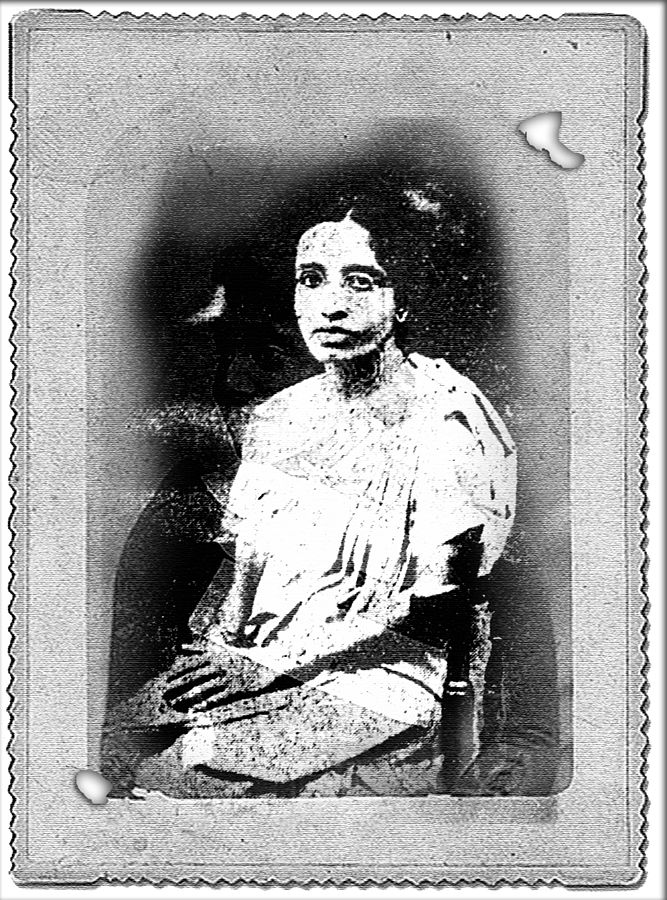
\includegraphics[width=0.4\textwidth,height=4cm]{Kulasthree_Chapter_four_pic10.jpg}
\end{center}
തൃശൂർജില്ലയിലെ കൂർക്കഞ്ചേരിയിൽ ജനിച്ചു. പ്രശസ്തനായ ഇ.കെ. അയ്യാക്കുട്ടി ജഡ്ജിയായിരുന്നു പിതാവ്. മദ്രാസിലെ ക്വീൻമേരീസ് കലാലയത്തിലും ലേഡി വെല്ലിങ്ടൺ കലാലയത്തിലും ഉന്നതവിദ്യാഭ്യാസം പൂർത്തിയാക്കിയശേഷം തൃശൂരിലെ വിവേകോദയം സ്കൂളിൽ അദ്ധ്യാപികയായി. പിൽക്കാലത്ത് ശ്രീലങ്കയിലെ ഒരു വിദ്യാലയത്തിലും ഒരു വർഷം പ്രവർത്തിക്കുകയുണ്ടായി. 1930ൽ സഹോദരൻ കെ. അയ്യപ്പനെ വിവാഹംചെയ്തു. ശ്രീനാരായണദർശനത്തെ വിപുലീകരിച്ച യുക്തിവാദിയായ അയ്യപ്പന്റെയൊപ്പം സാമൂഹ്യപരിവർത്തനപ്രവർത്തനങ്ങളിൽ തുല്യപങ്കാളിയായി പ്രവർത്തിച്ചു. സ്ത്രീ എന്ന വനിതാമാസികയുടെ പത്രാധിപരായിരുന്നു. 1956ൽ ജോലിയിൽനിന്നു വിരമിച്ചശേഷം ശ്രീനാരായണസേവികാസമാജം സ്ഥാപിച്ചു. 1988വരെ പൊതുജീവിതത്തിൽ സജീവസാന്നിദ്ധ്യമായിരുന്നു.


\end{tcolorbox}

\paragraph{}ഇത്തരത്തിൽ വാദിച്ച വനിതാപരിഷ്ക്കർത്താക്കളുടെ പരമ്പര, പക്ഷേ, പിൽക്കാലത്തു വികസിച്ചില്ലെന്നു പറയാം. സരസ്വതിയമ്മയുടേതായിരുന്നു അവസാനത്തെ ശബ്ദം. സാമൂഹ്യ-സാമ്പത്തികമായി പിന്നോക്കംനിൽക്കുന്ന സ്ത്രീകളെ തൊഴിൽനല്കി, കുടിൽവ്യവസായത്തിലൂടെ, 'ഉദ്ധരിക്കാനു'ള്ള ബാദ്ധ്യത മേലാളസ്ത്രീകൾക്കുണ്ടെന്ന് പറഞ്ഞുകൊണ്ട് മേലാളസ്ത്രീകളെ പരിഷ്ക്കർത്താവിന്റെ കുപ്പായമണിയിക്കാൻ ചിലർ ഉത്സാഹിച്ചിരുന്നു. ഈ പരിഷ്ക്കരണനിർദ്ദേശത്തിന് ഒരു പ്രത്യേകതയുണ്ടായിരുന്നു. മേൽവിവരിച്ച പുരുഷപരിഷ്ക്കർത്താവിന്റെ നിലയെ അപേക്ഷിച്ച് ദുർബലമായിരുന്നു ദരിദ്രസ്ത്രീകളെ ഉദ്ധരിക്കാൻ പണിപ്പെടേണ്ടവരായ സ്ത്രീപരിഷ്ക്കർത്താക്കളുടെ നില. പുരുഷനായ പരിഷ്ക്കർത്താവ് പരിപക്വവും പൂർണ്ണവുമായ വ്യക്തിത്വത്തിന്റെയുടമയായിയാണ് സങ്കൽപ്പിക്കപ്പെട്ടത് - ആ നിലയിൽനിന്നുകൊണ്ടാണ് അയാൾ സ്ത്രീയെ പരിഷ്ക്കരിക്കുന്നത്. എന്നാൽ തൊഴിൽപരിശീലനവുംമറ്റും നൽകി മറ്റുസ്ത്രീകളെ ഉയർത്തിക്കൊണ്ടുവരുന്ന സ്ത്രീയായ പരിഷ്ക്കർത്താവിന് അത്തരമൊരു നില കൽപ്പിക്കപ്പെടുന്നില്ല. മറിച്ച് സദാ ആത്മനിയന്ത്രണവും മേൽനോട്ടവും ഉണ്ടെങ്കിലേ സ്ത്രീ നേർവഴി നടക്കൂ എന്ന പരോക്ഷധാരണയും ഇത്തരം നിർദ്ദേശങ്ങളിലുണ്ടായിരുന്നു. കുടിൽവ്യവസായം ആരംഭിക്കുന്നതിലൂടെ സ്ത്രീ സ്വന്തം കുടുംബത്തിന്റെ സാമ്പത്തികസ്ഥിതി മെച്ചപ്പെടുത്തും; മറ്റുസ്ത്രീകളോടുള്ള തന്റെ കടമ നിർവ്വഹിക്കും തുടങ്ങിയ വാദങ്ങൾക്കുപുറമെ സ്ത്രീയുടെ ആത്മനിയന്ത്രണത്തെയും അച്ചടക്കത്തെയും ഇത്തരം പ്രവർത്തനങ്ങൾ പരിപോഷിപ്പിക്കുമെന്ന വാദവും വളരെ പ്രാധാന്യത്തോടെ ഉന്നയിക്കപ്പെട്ടു:

\begin{quotation}
...അവൾക്ക് (കുടിൽവ്യവസായത്തിലേർപ്പെടുന്ന വീട്ടമ്മയ്ക്ക്)സൽബുദ്ധി വർദ്ധിക്കുകയും ദുർബുദ്ധി കുറയുകയും ചെയ്യും. അലസമായ തലച്ചോറ് പിശാചിന്റെ പണിപ്പുരയാണല്ലോ... നല്ല കാര്യങ്ങളിൽ മനസ്സു പ്രവേശിപ്പിച്ചുകൊണ്ടാൽ അന്യജനങ്ങളുടെ ദൂഷ്യം ഉണ്ടാക്കുന്നതിനും തരമില്ലാതെവരുന്നത് എത്ര ഭാഗ്യമാണ്... സ്ത്രീകളുടെ തൊഴിലില്ലായ്മയെ പരിഹരിക്കുന്നതിനും അവർക്കു ക്ഷേമം വർദ്ധിപ്പിക്കുന്നതിനുമായി ആദായകരങ്ങളായ പ്രത്യേക പ്രവൃത്തികൾ അവരുടെ വാസനയ്ക്കും മാനത്തിനും മര്യാദയ്ക്കും പഠിപ്പിനും തക്കവണ്ണം കണ്ടുപിടിച്ച്, അവരെക്കൊണ്ട് ചെയ്യിപ്പിച്ച്, അവർ ഉണ്ടാക്കുന്ന സാധനങ്ങളെ വിറ്റഴിക്കുന്നിതിനുള്ള ഏർപ്പാടുചെയ്തു നടപ്പിൽവരുത്തുന്നത് നമ്മുടെ ഇടയിലുള്ള വിദുഷികളായ സ്ത്രീകളുടെ ഉത്തമകൃത്യങ്ങളാകുന്നു. 
\flushright{(എൽ. മീനാക്ഷിയമ്മ, 'സ്ത്രീകളുടെ തൊഴിലില്ലായ്മ', മഹിളാരത്നം 1(1), 1927-28)}

\end{quotation}

\paragraph{}ഇങ്ങനെ രണ്ടാംകിടയിൽ തളയ്ക്കപ്പെട്ടെങ്കിലും കീഴാളസ്ത്രീകളെക്കാൾ മുന്തിയസ്ഥാനം തങ്ങൾക്കുണ്ടെന്നതുകൊണ്ടുതന്നെ യാതൊരുവിധ ചോദ്യംചെയ്യലിനും മേലാളസ്ത്രീകൾ മുതിർന്നില്ല. ആദ്യകാലസ്ത്രീവാദത്തിന്റെ പരാജയങ്ങളിലൊന്നായിരുന്നു അത് - പരിഷ്ക്കരണവാദത്തെ പൂർണ്ണമായി തള്ളിക്കളയാൻ ആദ്യകാലസ്ത്രീവാദികളിൽ ചുരുക്കം ചിലർക്കേ കഴിഞ്ഞുള്ളൂ. ഫലമോ, മേലാള-കീഴാളസ്ത്രീകൾക്കിടയിൽ പുതിയ പിതൃമേധാവിത്വത്തോട് സാമ്യംപുലർത്തിയ അധികാരബന്ധം സങ്കൽപ്പിക്കപ്പെട്ടു. ആദ്യകാലകമ്യൂണിസ്റ്റ് എഴുത്തുകാർ, സാമൂഹ്യപ്രവർത്തകരായ വരേണ്യസ്ത്രീകളെ 'കൊച്ചമ്മമാ'രെന്ന് വിളിച്ചാക്ഷേപിച്ചത് വെറുതെയല്ല. തൊഴിലാളിസ്ത്രീകൾ വൻതോതിൽ സംഘടിതരായ 1940കളിൽ പൂർണ്ണപൗരത്വം അവർ പിടിച്ചെടുക്കുമെന്ന സ്വപ്നം യാഥാർത്ഥ്യമാകാൻപോകുന്നുവെന്ന തോന്നൽ പലർക്കുമുണ്ടായതിൽ അത്ഭുതമില്ല. പ്രത്യേകിച്ച് പരിഷ്ക്കരണമോ ഉദ്ധാരണമോ ഒന്നുംകൂടാതെതന്നെ പൂർണ്ണപൗരത്വത്തിന് തങ്ങൾ അർഹരാണെന്നും അത് തങ്ങളുടെ അവകാശമാണെന്നും തൊഴിലാളിവക്താക്കൾ പലരും പ്രഖ്യാപിച്ചു. (എന്നാൽ പരിഷ്ക്കരണത്തിന്റെ അംശങ്ങൾ പൂർണ്ണമായും ഒഴിവാക്കപ്പെട്ടില്ലെന്നത് മറ്റൊരു കാര്യം. തൊഴിലാളിപ്രസ്ഥാനത്തിന്റെ ഉന്നതതലങ്ങളിൽ ആ താത്പര്യം പ്രകടമായിരുന്നു). ആദ്യകാല സ്ത്രീവാദികൾക്കിടയിൽത്തന്നെ വ്യത്യസ്ത അഭിപ്രായക്കാരുണ്ടായിരുന്നുവെന്ന് സൂചിപ്പിച്ചുവല്ലോ - അത്തരം വ്യത്യസ്തതകൾ മുഴുവൻ അവഗണിക്കപ്പെട്ടു; ഒന്നുകിൽ 'കൊച്ചമ്മ' അല്ലെങ്കിൽ 'സൊസൈറ്റി ലേഡി' എന്നീ രണ്ടു പരിഹാസ്യകഥാപാത്രങ്ങളിലേക്ക് ആദ്യകാലസ്ത്രീവാദികൾ ന്യൂനീകരിക്കപ്പെട്ടു.

\paragraph{}'തറവാട്ടിൽ പിറന്നവളും' 'ചന്തപ്പെണ്ണും' തമ്മിലുള്ള അസമത്വം അങ്ങനെ നമ്മുടെ ഇക്കാലത്തും നിലനിൽക്കുന്നുണ്ട്. ജാതിവ്യവസ്ഥയെ മാറ്റിമറിച്ച കേരളീയനവോത്ഥാനം ഈ രണ്ടു സംവർഗ്ഗങ്ങളെയും 20-ാം നൂറ്റാണ്ടിൽ പുനഃസൃഷ്ടിച്ചതിനെക്കുറിച്ചാണ് ഈ അദ്ധ്യായത്തിൽ പറഞ്ഞത്. പരിഷ്ക്കരണവാദങ്ങളിലൂടെ വ്യാപകമായ ലിംഗമാന്യതയും ലിംഗാദർശവും 20-ാം നൂറ്റാണ്ടിൽ കൂടുതൽ ജനവിഭാഗങ്ങളിലേക്ക് വ്യാപിക്കുകയുണ്ടായി. ഒരു സമുദായത്തിന് സമൂഹത്തിൽ ഉയരണമെങ്കിൽ അതിലെ സ്ത്രീകൾ ഈ പുതിയ ലിംഗമാന്യതയ്ക്കു കീഴ്പ്പെടണമെന്ന അലിഖിതനിയമം ഇവിടെ പ്രാവർത്തികമായി. സ്ത്രീകൾക്ക് ഈ നവമാന്യതകൂടാതെ സമൂഹത്തിൽനിന്ന് സുരക്ഷ ലഭിക്കില്ലെന്നും വന്നു. നവമാന്യത നിർവ്വചിക്കുന്ന 'അടക്കമൊതുക്ക'ത്തിനുള്ളിൽ ജീവിക്കുന്നവളാണ് താനെന്ന് തെളിവു ഹാജരാക്കുന്ന സ്ത്രീക്കുമാത്രമേ ലൈംഗികാതിക്രമത്തിനെതിരെ ധൈര്യമായി പരാതിപ്പെടാൻ കഴിയൂ; കാരണം ആ തെളിവില്ലാതെ സമൂഹത്തെയും നീതിന്യായവ്യവസ്ഥയെയും സമീപിച്ചാൽ സംശയവും അപമാനവും ഏൽക്കേണ്ടിവരും. നവവരേണ്യ ലിംഗമാന്യതയെ അതിലംഘിച്ചവൾ എന്ന പേരുണ്ടായാൽമതി, ആ സ്ത്രീ പറയുന്നതെല്ലാം നുണയാണെന്ന് കണ്ണുമടച്ച് വിളിച്ചുപറയാൻ ആളുണ്ടാകും. 

\paragraph{}ജോലി ചെയ്യുന്നുവെങ്കിൽ അദ്ധ്യാപനം, ഓഫീസ്ജോലി മുതലായ 'മാന്യമായ തൊഴിലി'നുമാത്രമേ പോകാവൂ; ഭർത്താവ് എത്ര വലിയ മൂർഖനാണെങ്കിലും കഴിവതും സഹിച്ചും ക്ഷമിച്ചും വിവാഹിത എന്ന പേർ നിലനിർത്തിക്കൊള്ളണം; ഭർത്താവിനും മക്കൾക്കും അസൗകര്യമാണെങ്കിൽ ബുദ്ധിമുട്ടിനേടിയ ഉദ്യോഗം ഉപേക്ഷിച്ചുകൊള്ളണം; ബസ്സിൽ എത്രഭയങ്കര തിരക്കാണെങ്കിലും പുരുഷന്റെയടുത്ത് ഒഴിഞ്ഞുകിടക്കുന്ന സീറ്റിൽ ഇരുന്ന് 'ചാരിത്ര്യം' നഷ്ടമാക്കരുത്; നേരം ഇരുട്ടും മുമ്പ് വീട്ടിലെത്തണം; 'അനാശാസ്യങ്ങൾ'ക്കായി വീട്ടിനു പുറത്തിറങ്ങരുത്; സിനിമയ്ക്കോ പാർക്കിൽ നടക്കാനോ ഒറ്റയ്ക്കു പോകരുത്; 'മാന്യ'മായി വേഷം ധരിച്ചുകൊള്ളണം; വിയർത്തൊലിക്കുന്ന കാലാവസ്ഥയാണെങ്കിലും സർവ്വതും മൂടി നടന്നുകൊള്ളണം; പുരുഷന്മാരുമായി സൗഹൃദമരുത് - കൂട്ടുകാരികളോടുള്ള സമ്പർക്കംപോലും കണക്കിലധികം വേണ്ട; ശബ്ദമുയർത്തി സംസാരിക്കരുത്; പരസ്യമായി ഉറക്കെ ചിരിക്കരുത്; മുതിർന്നവരുടെയും മേലുദ്യോഗസ്ഥരുടെയും മുന്നിൽ അധികം ആത്മവിശ്വാസമരുത്; വീട്ടുജോലി ചെയ്യാൻ ഇഷ്ടമല്ലെങ്കിലും അതു പുറത്തു പറയരുത്; കുട്ടികളോട് വാത്സല്യമില്ലെങ്കിലും വിവാഹംകഴിഞ്ഞ് രണ്ടു വർഷത്തിനകം പ്രസവിച്ചിരിക്കണം... 'മാന്യത'യ്ക്കുവേണ്ടി മലയാളിസ്ത്രീ അനുസരിച്ചുവരുന്ന അസംഖ്യം നിയന്ത്രണങ്ങളിൽ ചിലതുമാത്രമേ ഇവിടെ പറഞ്ഞുള്ളു. 'ആത്മാഭിമാന'വും 'മാന്യത'യും രണ്ടാണെന്ന ബോധം എന്നുണ്ടാകുന്നോ അന്നേ ഈ കോട്ട തകരൂ. അതുവരെ 'സ്ത്രീത്വം' എന്ന ആദർശം ഈ കോട്ടയുടെ ആണിക്കല്ലായി തുടരും.

\section{കൂടുതൽ ആലോചനയ്ക്ക്}

സ്ത്രീപുരുഷവ്യത്യാസം പ്രകൃതിനിർണ്ണിതവും അചഞ്ചലവുമാണെന്ന വിശ്വാസത്തെ സ്ത്രീപക്ഷചരിത്രരചന എക്കാലവും ചോദ്യം ചെയ്തിട്ടുണ്ട്. മാറിവരുന്ന സാമൂഹ്യ-രാഷ്ട്രീയ സാഹചര്യങ്ങളുടെ സമ്മർദ്ദത്തിൽ 'സ്ത്രീത്വം', 'പുരുഷത്വം' മുതലായ ആശയങ്ങളും അവയോടു ചേർന്നു നിൽക്കുന്ന പ്രയോഗങ്ങളും മാറിവരുന്നതെങ്ങനെ എന്ന് അന്വേഷിക്കുന്ന വിമർശനാത്മക 'ലിംഗചരിത്രരചന'യുടെ ഉൾക്കാഴ്ചകളാണ് ഈ അദ്ധ്യായത്തിൽ പ്രയോഗിച്ചിട്ടുള്ളത് - സ്ത്രീത്വത്തിന് കൂടുതൽ ഊന്നൽ നൽകിയിരിക്കുന്നുവെന്നു മാത്രം (പുരുഷത്വത്തെക്കുറിച്ചുള്ള ചർച്ചകളുടെ ചരിത്രം ഇനിയും പഠിക്കേണ്ടിയിരിക്കുന്നു). എങ്കിലും 'പുരുഷനായ പരിഷ്ക്കർത്താവി'നെക്കുറിച്ചു പറഞ്ഞിടത്ത് പുതിയ പുരുഷാദർശങ്ങളെക്കുറിച്ച് ഒരു സൂചനയുണ്ട്. സാമൂഹ്യപരിഷ്ക്കരണം ഒരു 'ലിംഗവൽകൃതപ്രക്രിയ'യാണെന്ന സൂചനയാണ് പൊതുവെ ഈ വിശകലനത്തിൽനിന്നു ലഭിക്കുന്നത്. വാസ്തവത്തിൽ 'പുരുഷനായ പരിഷ്ക്കർത്താവ്' ഒരു അനിവാര്യതയായിരുന്നോ? സ്ത്രീകളെ (ആധുവിക ജീവിതരീതികളിൽനിന്ന് അകലെയായിരുന്ന മറ്റു ജനങ്ങളെയും) പൂർണ്ണ പൗരത്വത്തിലെത്തിക്കാൻ മറ്റു വഴികളുണ്ടായിരുന്നില്ലേ? പരിഷ്ക്കർത്താവ്-പരിഷ്ക്കരണവസ്തു എന്ന അസമബന്ധമല്ലാതെ മറ്റു മാർഗ്ഗങ്ങൾ നമുക്ക് വിഭാവനംചെയ്യാൻ കഴിയുമോ?

ഒരേ സമയം പലതിനെയും ഉൾക്കൊള്ളുന്നതാണ് ചരിത്രം - ജനങ്ങൾ, സ്ഥലങ്ങൾ, വസ്തുക്കൾ, ആശയങ്ങൾ, സംഭവങ്ങൾ, ഓർമ്മകൾ, ഐതിഹ്യങ്ങൾ, കഥകൾ ഇവയെയെല്ലാം ഒരേ ചരടിൽ കോർത്തിണക്കാൻ ഇതിനു കഴിയും. ചരിത്രത്തോട് എനിക്കു തോന്നിയ ഇഷ്ടത്തിനു കാരണങ്ങൾ പലതാണ്; ഞാൻ ചരിത്രരചനയ്ക്കായി സ്വീകരിച്ചിട്ടുള്ള മാർഗ്ഗങ്ങളും കാലത്തിൽ മാറിയിട്ടുണ്ട്. എങ്കിലും ഭൂതകാലത്തിന്റെ വശ്യമായ നിഗൂഢത, അതിന്റെ സവിശേഷമായ തീർച്ചയില്ലായ്മ - നമ്മെ നിശ്ചയമായും പിടിച്ചിരുത്തുകയും കുഴയ്ക്കുകയും ചെയ്യുന്ന ആ തീർച്ചയില്ലായ്മ - ചരിത്രപഠനത്തിലേക്ക് എന്നെ ആകർഷിച്ച മുഖ്യഘടകങ്ങളിലൊന്നായിരുന്നു. ഡൽഹിയിൽ ജനിച്ചുവളർന്ന കുട്ടിയെന്ന നിലയ്ക്ക് ചരിത്രവുമായുള്ള എന്റെ ആദ്യത്തെ ഇടപെടൽ ഇവിടത്തെ ചരിത്രസ്മാരകങ്ങളിലൂടെയായിരുന്നു - മറ്റൊരു കാലത്തെ, മറ്റു ജീവിതങ്ങളെ വിളിച്ചോതുന്ന ഇടങ്ങൾ. ഞാനൊരിക്കലും ഡൽഹിയെ 'പഠിച്ചിട്ടില്ല'; കെട്ടിടങ്ങളും ഇടങ്ങളും മനുഷ്യർ ജീവിച്ചുതീർക്കുന്ന സാമൂഹ്യചരിത്രവും തമ്മിലുള്ള ബന്ധത്തെക്കുറിച്ച് അടുത്തകാലത്തുമാത്രമാണ് ഞാൻ അന്വേഷണമാരഭിച്ചിട്ടുള്ളത്. എങ്കിലും ഇവിടെപ്പറഞ്ഞ ആ ആദ്യസമാഗമം തുറന്നുതന്ന ചോദ്യങ്ങൾ എല്ലായ്പ്പോഴും എന്റെയൊപ്പമുണ്ടായിട്ടുണ്ട്. അതുകൊണ്ടുതന്നെ ഭൂതകാലത്തെ പ്രതിനിധീകരിക്കുന്ന രൂപങ്ങളായ നോവലുകൾ, ചിത്രങ്ങൾ, ഫോട്ടോഗ്രാഫുകൾ തുടങ്ങിയവയായാലും ശരി, വിവാഹം, ചാർച്ചാബന്ധങ്ങൾ മുതലായ അമൂർത്തസാമൂഹ്യബന്ധങ്ങളായാലും ശരി, ഭൂതകാലം (എന്നെ) പിടിച്ചിരുത്തി ചിന്തിപ്പിക്കുന്നു; എന്നാൽ എളുപ്പമങ്ങ് വിശദീകരിച്ചുകളയാനനുവദിക്കുന്ന ചട്ടക്കൂടുകളൊന്നും അതെനിക്കു തരുന്നുമില്ല! കഴിഞ്ഞ ദശകങ്ങളിൽ ചരിത്രപഠനത്തിൽ നാം പലതരം ഉപകരണങ്ങളും രീതികളും അപഗ്രഥനത്തിനായുപയോഗിച്ചിട്ടുണ്ട്; ചരിത്രം പലവിധത്തിൽ പഠിക്കപ്പെട്ടിട്ടുണ്ട്. ഇന്നാകട്ടെ, നമ്മുടെ ഇന്നത്തെ ചോദ്യങ്ങളുടെ മാറ്റൊലികൾ ഭൂതകാലത്തെ പഠിക്കാനുള്ള ഏറ്റവുംനല്ല മാർഗ്ഗമേതെന്ന വിഷയത്തെച്ചൊല്ലി നാം നടത്തുന്ന രീതിശാസ്ത്രചർച്ചകൾക്കു പിന്നിൽ മുഴങ്ങിക്കേൾക്കുന്നുണ്ടെന്ന കാര്യത്തെക്കുറിച്ച് ആർക്കും അഭിപ്രായവ്യത്യാസമുണ്ടാകാനിടയില്ല. ചരിത്രപഠനത്തിന്റെ ഒടുവിൽ ഏതൊ 'സനാതനസത്യം' എന്നെ കാത്തിരിക്കുന്നുവെന്ന ധാരണ ഞാൻ ഉപേക്ഷിച്ചിട്ട് കാലം കുറേയായി. എങ്കിലും ഓരോ പുതിയ പഠനവും ഭൂതകാലത്തിന്റെ ഇതുവരെ കാണാത്ത തുണ്ടുകളിലേക്കാണു തുറക്കുന്നത്. ഓരോ പഠനവും സമകാലികജീവിതത്തിന്റെ വ്യവസ്ഥകളെക്കുറിച്ചും അവസ്ഥകളെക്കുറിച്ചും നമ്മെ വീണ്ടുമാലോചിക്കാൻ പ്രേരിപ്പിക്കുന്നുമുണ്ട്. 

\section{കേരളത്തിന്റെ ചരിത്രകാരികൾ: ജി അരുണിമ}
\begin{center}
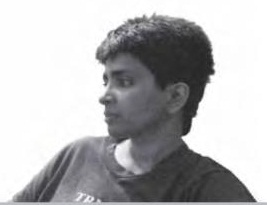
\includegraphics[width=0.4\textwidth,height=4cm]{Kulasthree_Chapter_four_pic11.jpg}
\end{center}
\paragraph{}ജി. അരുണിമ ഡൽഹിയിലെ ജവഹർലാൽ നെഹ്രു സർവ്വകലാശാലയിലെ സ്കൂൾ ഒഫ് സോഷ്യൽ സയൻസിൽ പ്രവർത്തിച്ചുവരുന്ന സ്ത്രീപഠന പ്രോഗ്രാമിൽ ചരിത്രകാരിയാണ്. കേരളത്തിന്റെ സാമൂഹിക-സാംസ്കാരികചരിത്രത്തെക്കുറിച്ച് ധാരാളം എഴുതിയിട്ടുണ്ട്. മലയാളിസമൂഹത്തിന്റെ കുടുംബ-ചാർച്ചാബന്ധങ്ങളെപ്പറ്റി ഗവേഷണംനടത്തുകയും ചെയ്തിട്ടുണ്ട്. സാംസ്കാരിക നിർമ്മാണമേഖലയെക്കുറിച്ച് - സാഹിത്യം, ചിത്രകല, ഫോട്ടോഗ്രഫി, അടുത്തകാലത്തായി സിനിമ എന്നിവയെപ്പറ്റിയും മതത്തെപ്പറിയും (വിശേഷിച്ച് വിശ്വാസവ്യവസ്ഥകൾ, സ്വത്വരൂപീകരണം എന്നിവയുമായി ബന്ധപ്പെടുത്തി) അവർ എഴുതുന്നു. There comes papa: Colonialism and the Transformation of Matriliny in Kerala (2003) ആണ് അവരുടെ പ്രധാനപ്രസിദ്ധീകരണം



